\documentclass[italian,10pt]{beamer}

\usetheme[secheader]{Madrid}
\usecolortheme{beaver}
\setbeamertemplate{navigation symbols}{}
\setbeamertemplate{footline}[frame number]
\setbeamertemplate{blocks}[rounded][shadow=true]
\setbeamersize{text margin left=1.2em, text margin right=1.2em}

\usepackage[italian]{babel}
\usepackage[utf8]{inputenc}
\usepackage[T1]{fontenc}
\usepackage{lmodern}
\usepackage{amsmath,amssymb}
\usepackage{graphicx}
\usepackage{booktabs}
\usepackage{multirow}
\usepackage{siunitx}
\usepackage{hyperref}
\usepackage{subfig}
\usepackage{tikz}
\usepackage{caption}
\usepackage{xcolor}
\definecolor{darkblue}{RGB}{16,55,110}
\definecolor{unired}{RGB}{200,40,40}

\setbeamercolor{title}{fg=unired}
\setbeamercolor{frametitle}{fg=darkblue}
\setbeamercolor{structure}{fg=darkblue}
\setbeamercolor{block title}{bg=darkblue,fg=white}
\setbeamercolor{block body}{bg=gray!10}

\newcommand{\upgreen}{\textcolor{green!50!black}{$\blacktriangle$}}
\newcommand{\downred}{\textcolor{red}{$\blacktriangledown$}}

\title[CI -- Deblur \& Denoise LBC]{\textbf{Computational Imaging}\\Deblur e Denoise di Immagini\\di Citologia Cervicale LBC}
\subtitle{Progetto -- Gruppo R}
\author[Castaldi, Fusco]{\textbf{Francesco Castaldi}\; \textcolor{gray}{|}\; \textbf{Paolo Fusco}}
\institute[DISI -- UniBO]{Dipartimento di Informatica -- Scienza e Ingegneria\\Universita di Bologna}
\date{A.A. 2025/2026}
\titlegraphic{
\includegraphics[width=0.22\textwidth]{figures/unibo_logo.png}}
\logo{
\includegraphics[width=0.05\textwidth]{figures/unibo_logo.png}}

\begin{document}

\begin{frame}[plain]
  \titlepage
  \vspace{-0.5cm}
  \begin{center}
    \small\href{https://github.com/FrancescoCastaldi/ci-cervical-lbc}{github.com/FrancescoCastaldi/ci-cervical-lbc}
  \end{center}
\end{frame}

\section{Descrizione del Progetto}

\begin{frame}{Problema Inverso}
  \begin{block}{Task}
    Data un'immagine di citologia cervicale degradata da \textbf{blur gaussiano} e \textbf{rumore AWGN}, stimare l'immagine originale.
  \end{block}
  \begin{equation*}
    y = \mathcal{H}(x) + n
  \end{equation*}
  \begin{itemize}
    \item $x$: immagine originale (ground truth, sconosciuta)
    \item $\mathcal{H}$: blur gaussiano ($\sigma=2$, kernel $9\times9$)
    \item $n$: AWGN con $\sigma_n \in \{0.005, 0.01, 0.05, 0.1\}$
    \item $y$: osservazione degradata
  \end{itemize}
  \begin{alertblock}{Problema Mal Posto (Ill-Posed)}
    Infinite soluzioni $x$ compatibili con $y$. Servono \textbf{regolarizzazioni} (TV) o \textbf{prior appresi} (UNet, DiffPIR).
  \end{alertblock}
\end{frame}

\begin{frame}{Metodi Scelti}
  \begin{center}\small Gruppo di 2 studenti $\to$ 3 metodi su 4 (escluso Weighted TV)\end{center}
  \begin{columns}[t]
    \column{0.33\textwidth}
      \begin{block}{Variazionale}
        \centering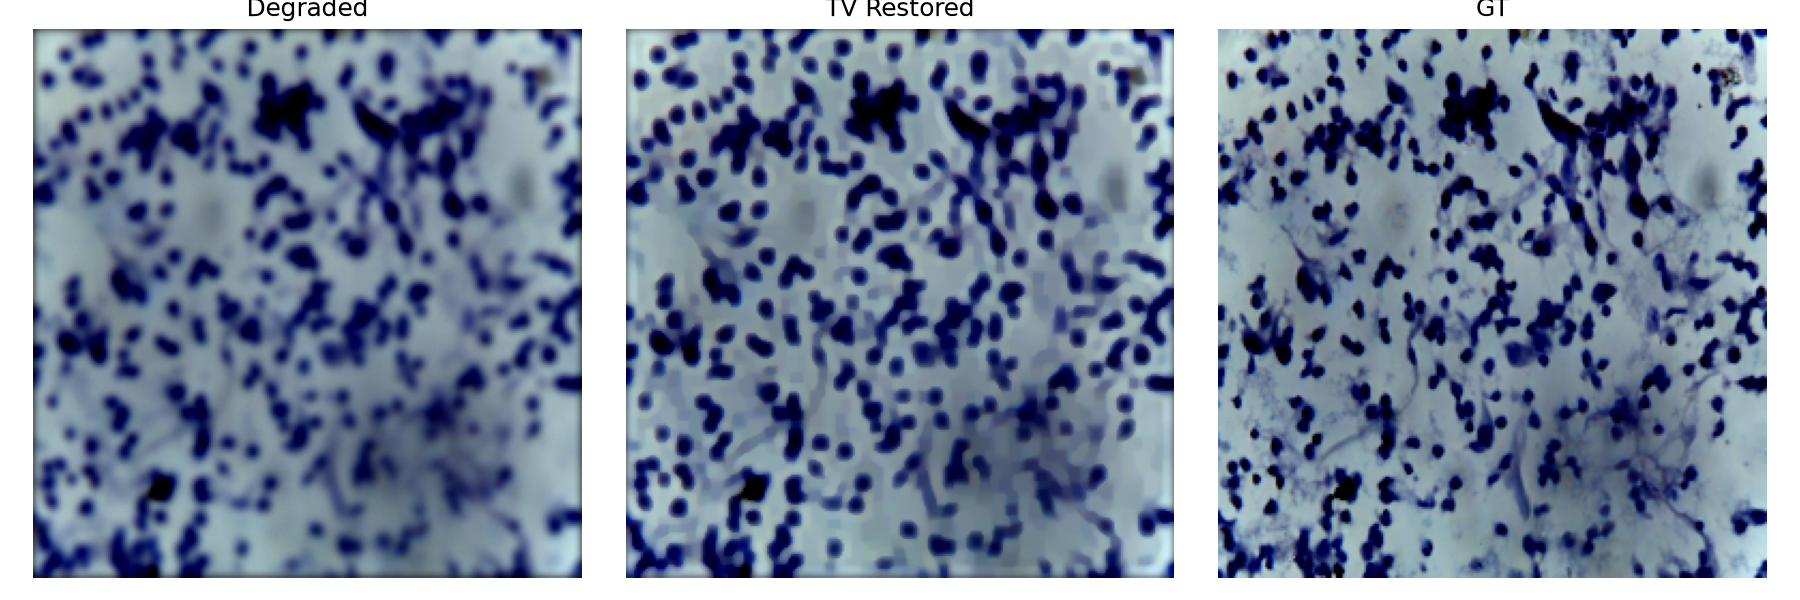
\includegraphics[height=1.1cm]{../results/tv/qualitative/noise_0.005_sample0.png}\\[0.05cm]
        \textbf{Total Variation}
        \begin{itemize}\small
          \item $\lambda=0.005$, Adam 150 iter
        \end{itemize}
      \end{block}
    \column{0.33\textwidth}
      \begin{block}{Deep Learning}
        \centering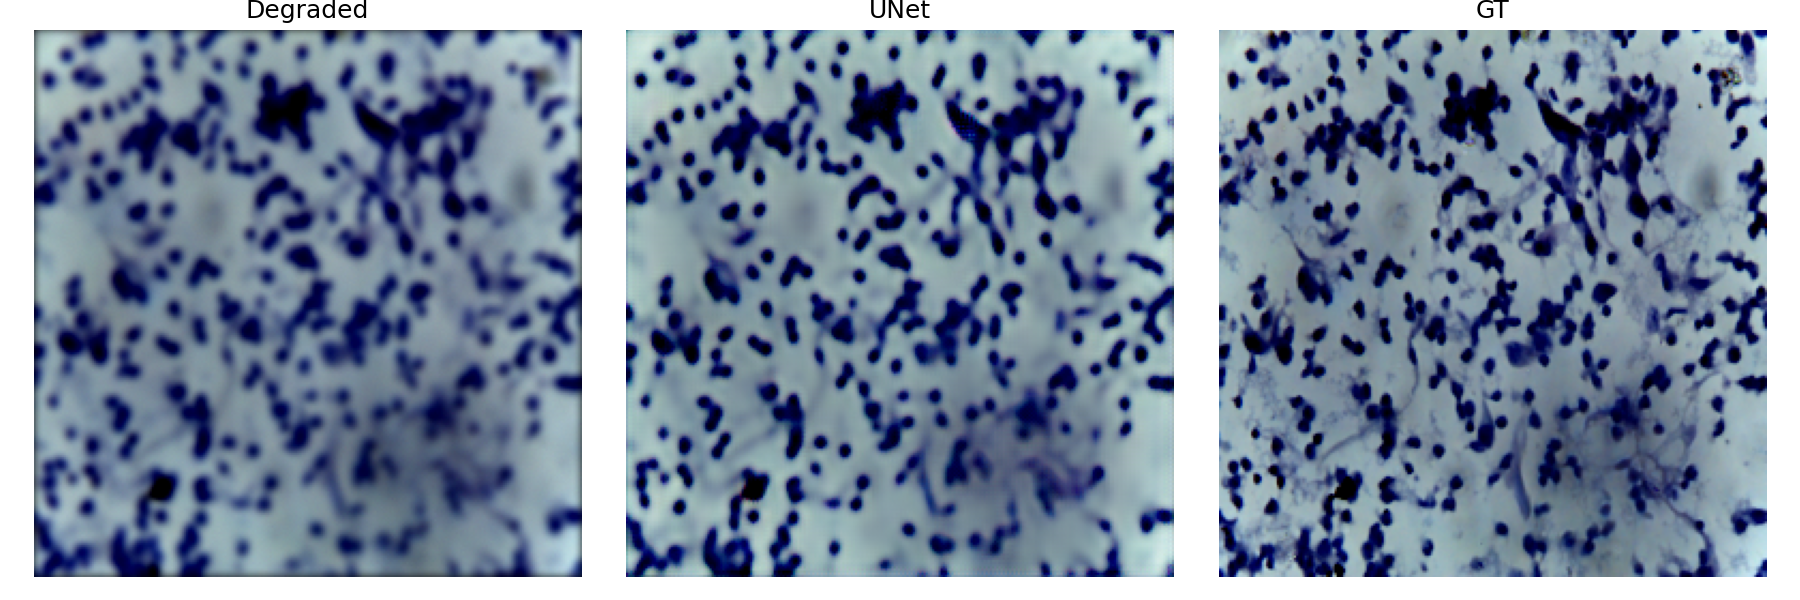
\includegraphics[height=1.1cm]{../results/unet/qualitative/noise_0.005_sample0.png}\\[0.05cm]
        \textbf{UNet}
        \begin{itemize}\small
          \item Encoder-Decoder, MSE+Adam
        \end{itemize}
      \end{block}
    \column{0.33\textwidth}
      \begin{block}{Generativo}
        \centering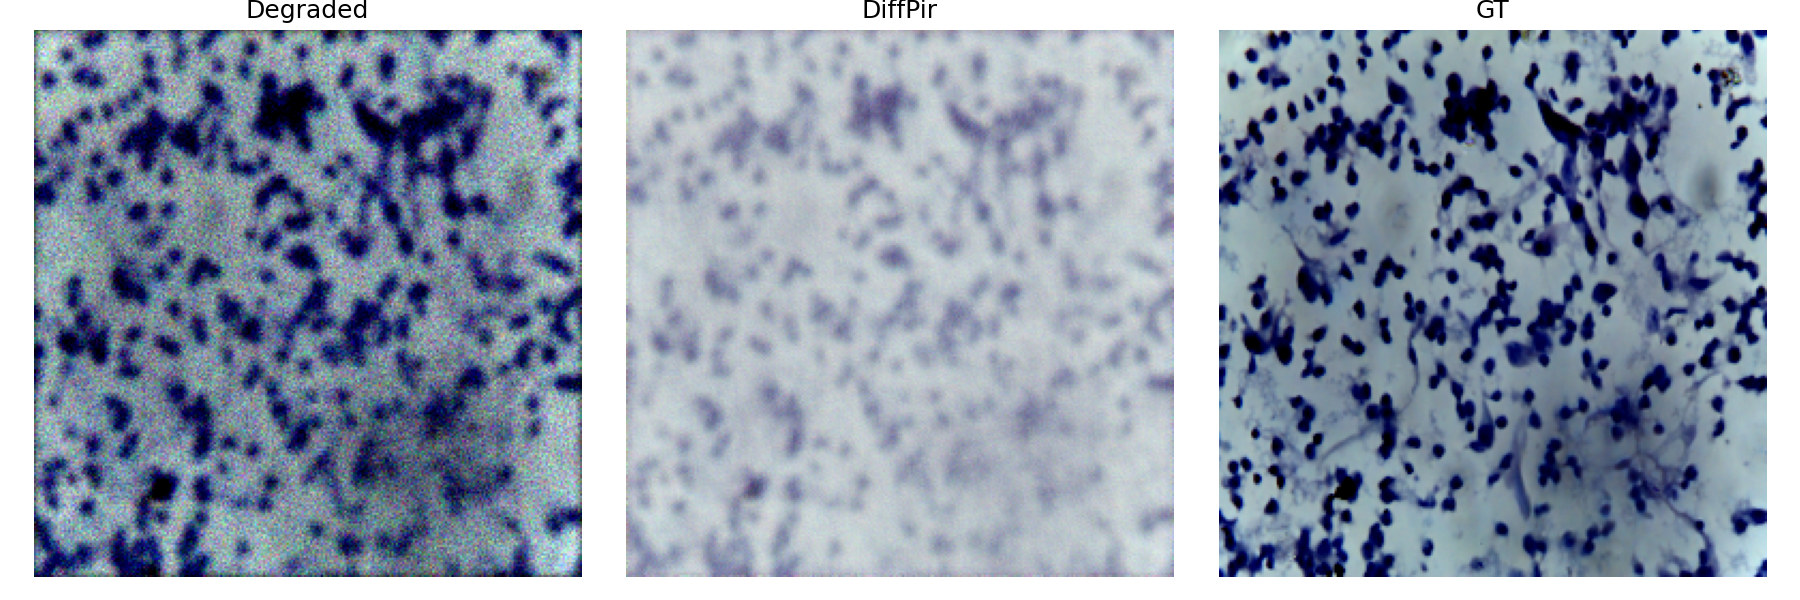
\includegraphics[height=1.1cm]{../results/diffpir/qualitative/noise_0.1_sample0.png}\\[0.05cm]
        \textbf{DiffPIR}
        \begin{itemize}\small
          \item DDPM+LightUNet, FFT fidelity
        \end{itemize}
      \end{block}
  \end{columns}
\end{frame}

\section{Dataset}

\begin{frame}{Mendeley LBC Cervical Cancer}
  \begin{columns}
    \column{0.55\textwidth}
      \begin{itemize}
        \item \textbf{962 immagini} di citologia cervicale
        \item Originali $2048\times1536$, \textbf{resize} a $256\times256$
        \item Normalizzazione in $[-1,1]$
      \end{itemize}
      \begin{block}{Classi diagnostiche}
        \begin{tabular}{lrc}\toprule
          \textbf{Classe} & \textbf{N} & \textbf{\%}\\\midrule
          NILM & 612 & 63.6\%\\
          HSIL & 163 & 16.9\%\\
          LSIL & 113 & 11.7\%\\
          SCC  & 74  & 7.7\%\\\bottomrule
        \end{tabular}
      \end{block}
    \column{0.45\textwidth}
      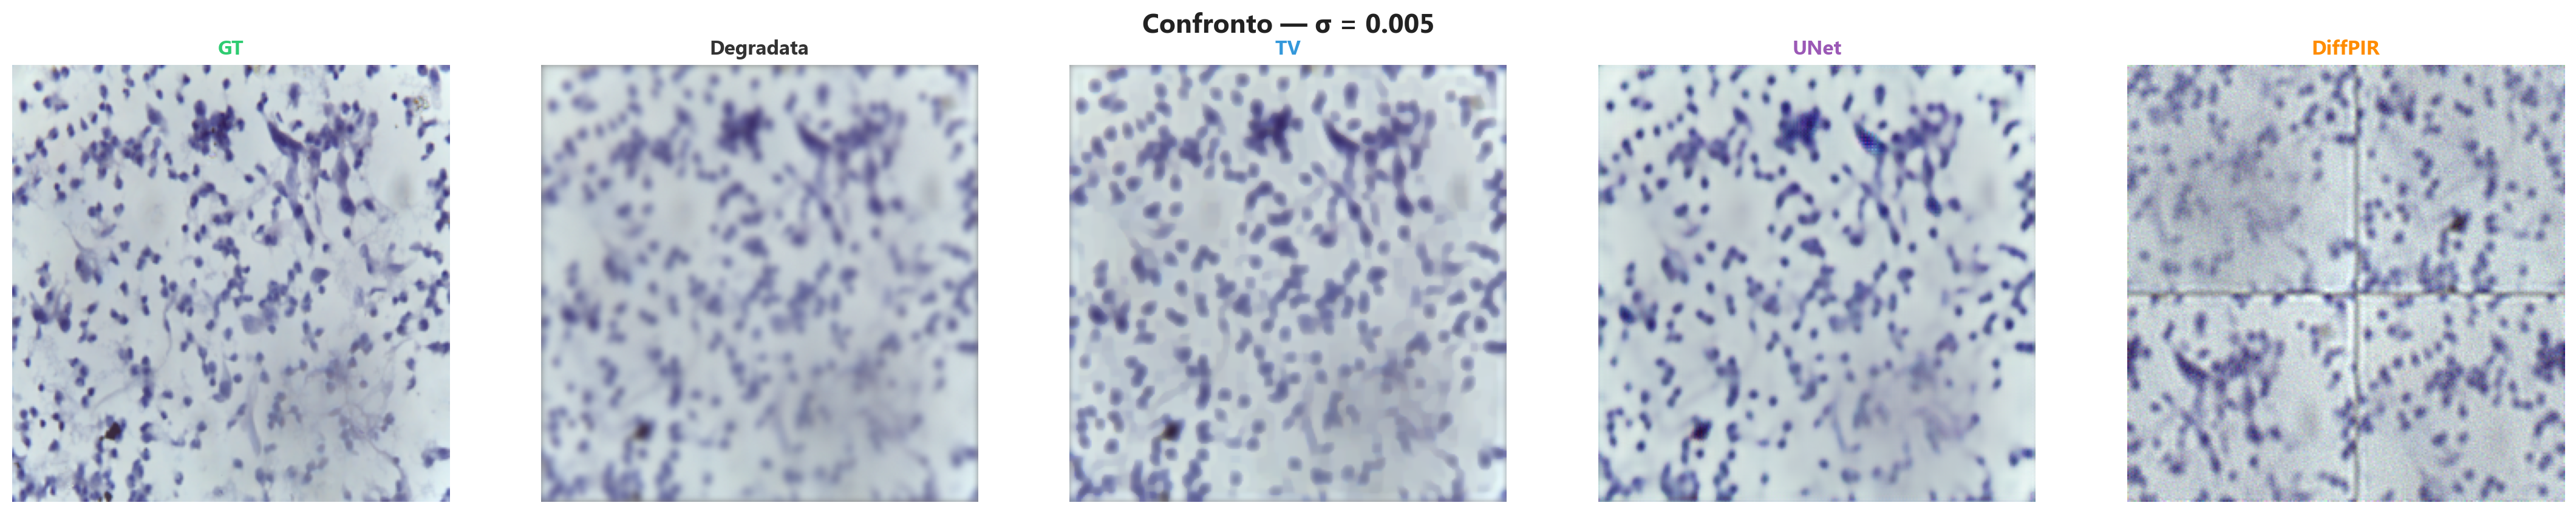
\includegraphics[width=\textwidth]{../results/qualitative_slides/noise_0.005_comparison.png}
  \end{columns}
\end{frame}

\begin{frame}{Preprocessing e Split}
  \begin{block}{Pipeline}
    \begin{tabular}{lll}\toprule
      \textbf{Passo} & \textbf{Operazione} & \textbf{Output}\\\midrule
      1 & Resize bilineare $2048\to256$ & $256\times256$\\
      2 & ToTensor $[0,255]\to[0,1]$ & float32\\
      3 & Normalizzazione $(x-0.5)/0.5$ & $[-1,1]$\\
      4 & Split stratificato 70/15/15 & train/val/test\\\bottomrule
    \end{tabular}
  \end{block}
  \begin{columns}
    \column{0.5\textwidth}
      \begin{block}{Suddivisione}
        \begin{tabular}{lrc}\toprule
          \textbf{Split} & \textbf{\%} & \textbf{Immagini}\\\midrule
          Training  & 70\% & 673\\
          Validation & 15\% & 144\\
          Test      & 15\% & 145\\\bottomrule
        \end{tabular}
      \end{block}
    \column{0.5\textwidth}
      \begin{itemize}
        \item Seed fisso 42
        \item Stratificato per classe
        \item Stesso test set per tutti
      \end{itemize}
  \end{columns}
\end{frame}

\section{Setup Sperimentale}

\begin{frame}{Degradazione}
  \begin{block}{Parametri identici per tutti i metodi}
    \begin{columns}
      \column{0.5\textwidth}
        \centering\textbf{Blur Gaussiano}\\[0.1cm]
        $\sigma=2$, kernel $9\times9$
      \column{0.5\textwidth}
        \centering\textbf{AWGN}\\[0.1cm]
        $\sigma_n\in\{0.005,0.01,0.05,0.1\}$
    \end{columns}
  \end{block}
  \vspace{0.15cm}
  \begin{columns}
    \column{0.45\textwidth}
      \textbf{Pipeline di degradazione:}
      \begin{enumerate}\small
        \item Applica blur gaussiano $H$ all'immagine GT $x$
        \item Aggiungi rumore AWGN $n$ con deviazione $\sigma_n$
        \item Clamping in $[-1,1]$
      \end{enumerate}
      \vspace{0.1cm}
      \begin{equation*}
        y = \mathcal{H}(x) + n
      \end{equation*}
      \vspace{0.1cm}
      \begin{itemize}\small
        \item Pipeline unica per tutti i metodi
        \item Seed 42 per riproducibilit\`a
      \end{itemize}
    \column{0.55\textwidth}
      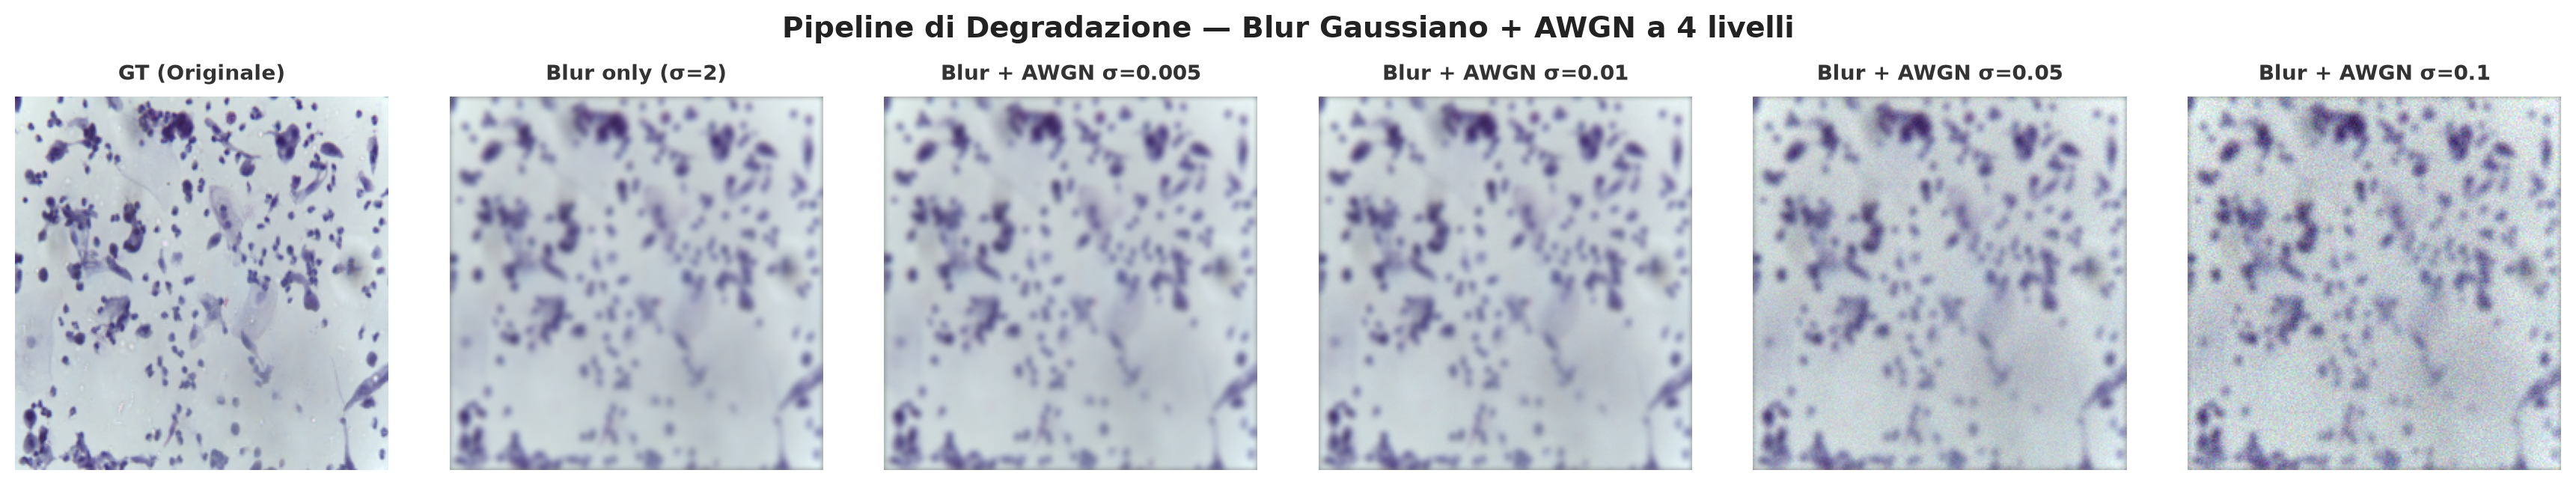
\includegraphics[width=\textwidth]{../results/qualitative_slides/noise_strip_crops.png}
  \end{columns}
\end{frame}

\section{Total Variation -- Paolo}

\begin{frame}{Total Variation -- Teoria}
  \begin{block}{Modello variazionale}
    \begin{equation*}
      \hat{x} = \arg\min_x \underbrace{\|H*x - y\|_2^2}_{\text{data fidelity}} + \lambda \cdot \underbrace{TV(x)}_{\text{regolarizzazione}}
    \end{equation*}
  \end{block}
  \vspace{0.2cm}
  \textbf{Total Variation}: somma delle differenze tra pixel adiacenti
  \begin{equation*}
    TV(x) = \sum_{i,j} |x_{i+1,j} - x_{i,j}| + |x_{i,j+1} - x_{i,j}|
  \end{equation*}
  \vspace{0.2cm}
  \begin{itemize}
    \item Preserva i bordi, rimuove il rumore
    \item Effetto \textit{staircasing} a $\lambda$ troppo alto
  \end{itemize}
  \vspace{0.2cm}
  \begin{block}{Parametri}
    \begin{tabular}{ll}
      $\lambda_{reg}=0.005$ & bilanciamento ottimale \\
      Ottimizzatore & Adam ($lr=0.001$) \\
      Iterazioni & 150 \\
      Clamping & $[-1,1]$ dopo ogni step \\
    \end{tabular}
  \end{block}
\end{frame}

\begin{frame}{Total Variation -- Algoritmo}
  \begin{columns}
    \column{0.53\textwidth}
      \textbf{Pseudo-codice:}
      \vspace{0.15cm}
      \begin{enumerate}
        \item $x \gets y$, $\lambda \gets 0.005$
        \item Ottimizzatore Adam ($lr = 10^{-3}$)
        \item \textbf{for} $i = 1$ \textbf{to} $150$ \textbf{do}
        \item \hspace{0.5cm}$x_{blur} \gets H * x$
        \item \hspace{0.5cm}$\mathcal{L} \gets \|x_{blur} - y\|_2^2 + \lambda \cdot TV(x)$
        \item \hspace{0.5cm}$\nabla_x\mathcal{L} \gets$ backpropagation
        \item \hspace{0.5cm}$x \gets$ AdamStep$(x, \nabla_x\mathcal{L})$
        \item \hspace{0.5cm}$x \gets \text{clamp}(x, -1, 1)$
        \item \textbf{end for}
        \item \textbf{return} $x$
      \end{enumerate}
    \column{0.47\textwidth}
      \small
      \textbf{TV Loss:}
      \begin{equation*}
        TV(x) = \sum_{i,j} |x_{i+1,j} - x_{i,j}| + |x_{i,j+1} - x_{i,j}|
      \end{equation*}
      \vspace{0.2cm}
      \textbf{Ciclo di ottimizzazione:}
      \begin{enumerate}
        \item Calcola $H*x$ (blur)\\\strut
        \item Loss: fidelity + regolarizzazione\\\strut
        \item Backpropagation\\\strut
        \item Step Adam\\\strut
        \item Clamp in $[-1,1]$
      \end{enumerate}
      \vspace{0.2cm}
      \textbf{Scelta di $\lambda$:}
      \begin{itemize}
        \item $\lambda=0.1$: staircasing
        \item $\lambda=0.001$: rumore residuo
        \item $\lambda=0.005$: bilanciamento ottimale
      \end{itemize}
  \end{columns}
\end{frame}

\begin{frame}{Total Variation -- Risultati}
  \begin{columns}
    \column{0.5\textwidth}
      \textbf{PSNR e SSIM su 145 immagini test}
      \vspace{0.2cm}
      \begin{tabular}{l|cc}\toprule
        $\sigma_n$ & \textbf{PSNR} & \textbf{SSIM}\\\midrule
        0.005 & \textbf{32.09} & \textbf{0.911}\\
        0.01  & \textbf{32.04} & \textbf{0.909}\\
        0.05  & 30.42 & 0.837\\
        0.1   & 26.54 & 0.586\\\bottomrule
      \end{tabular}
      \vspace{0.3cm}
      \begin{itemize}
        \item Eccellente a basso rumore (PSNR $>$ 32 dB)
        \item Degrado progressivo col rumore
        \item Staircasing visibile a $\sigma_n=0.1$
      \end{itemize}
    \column{0.5\textwidth}
      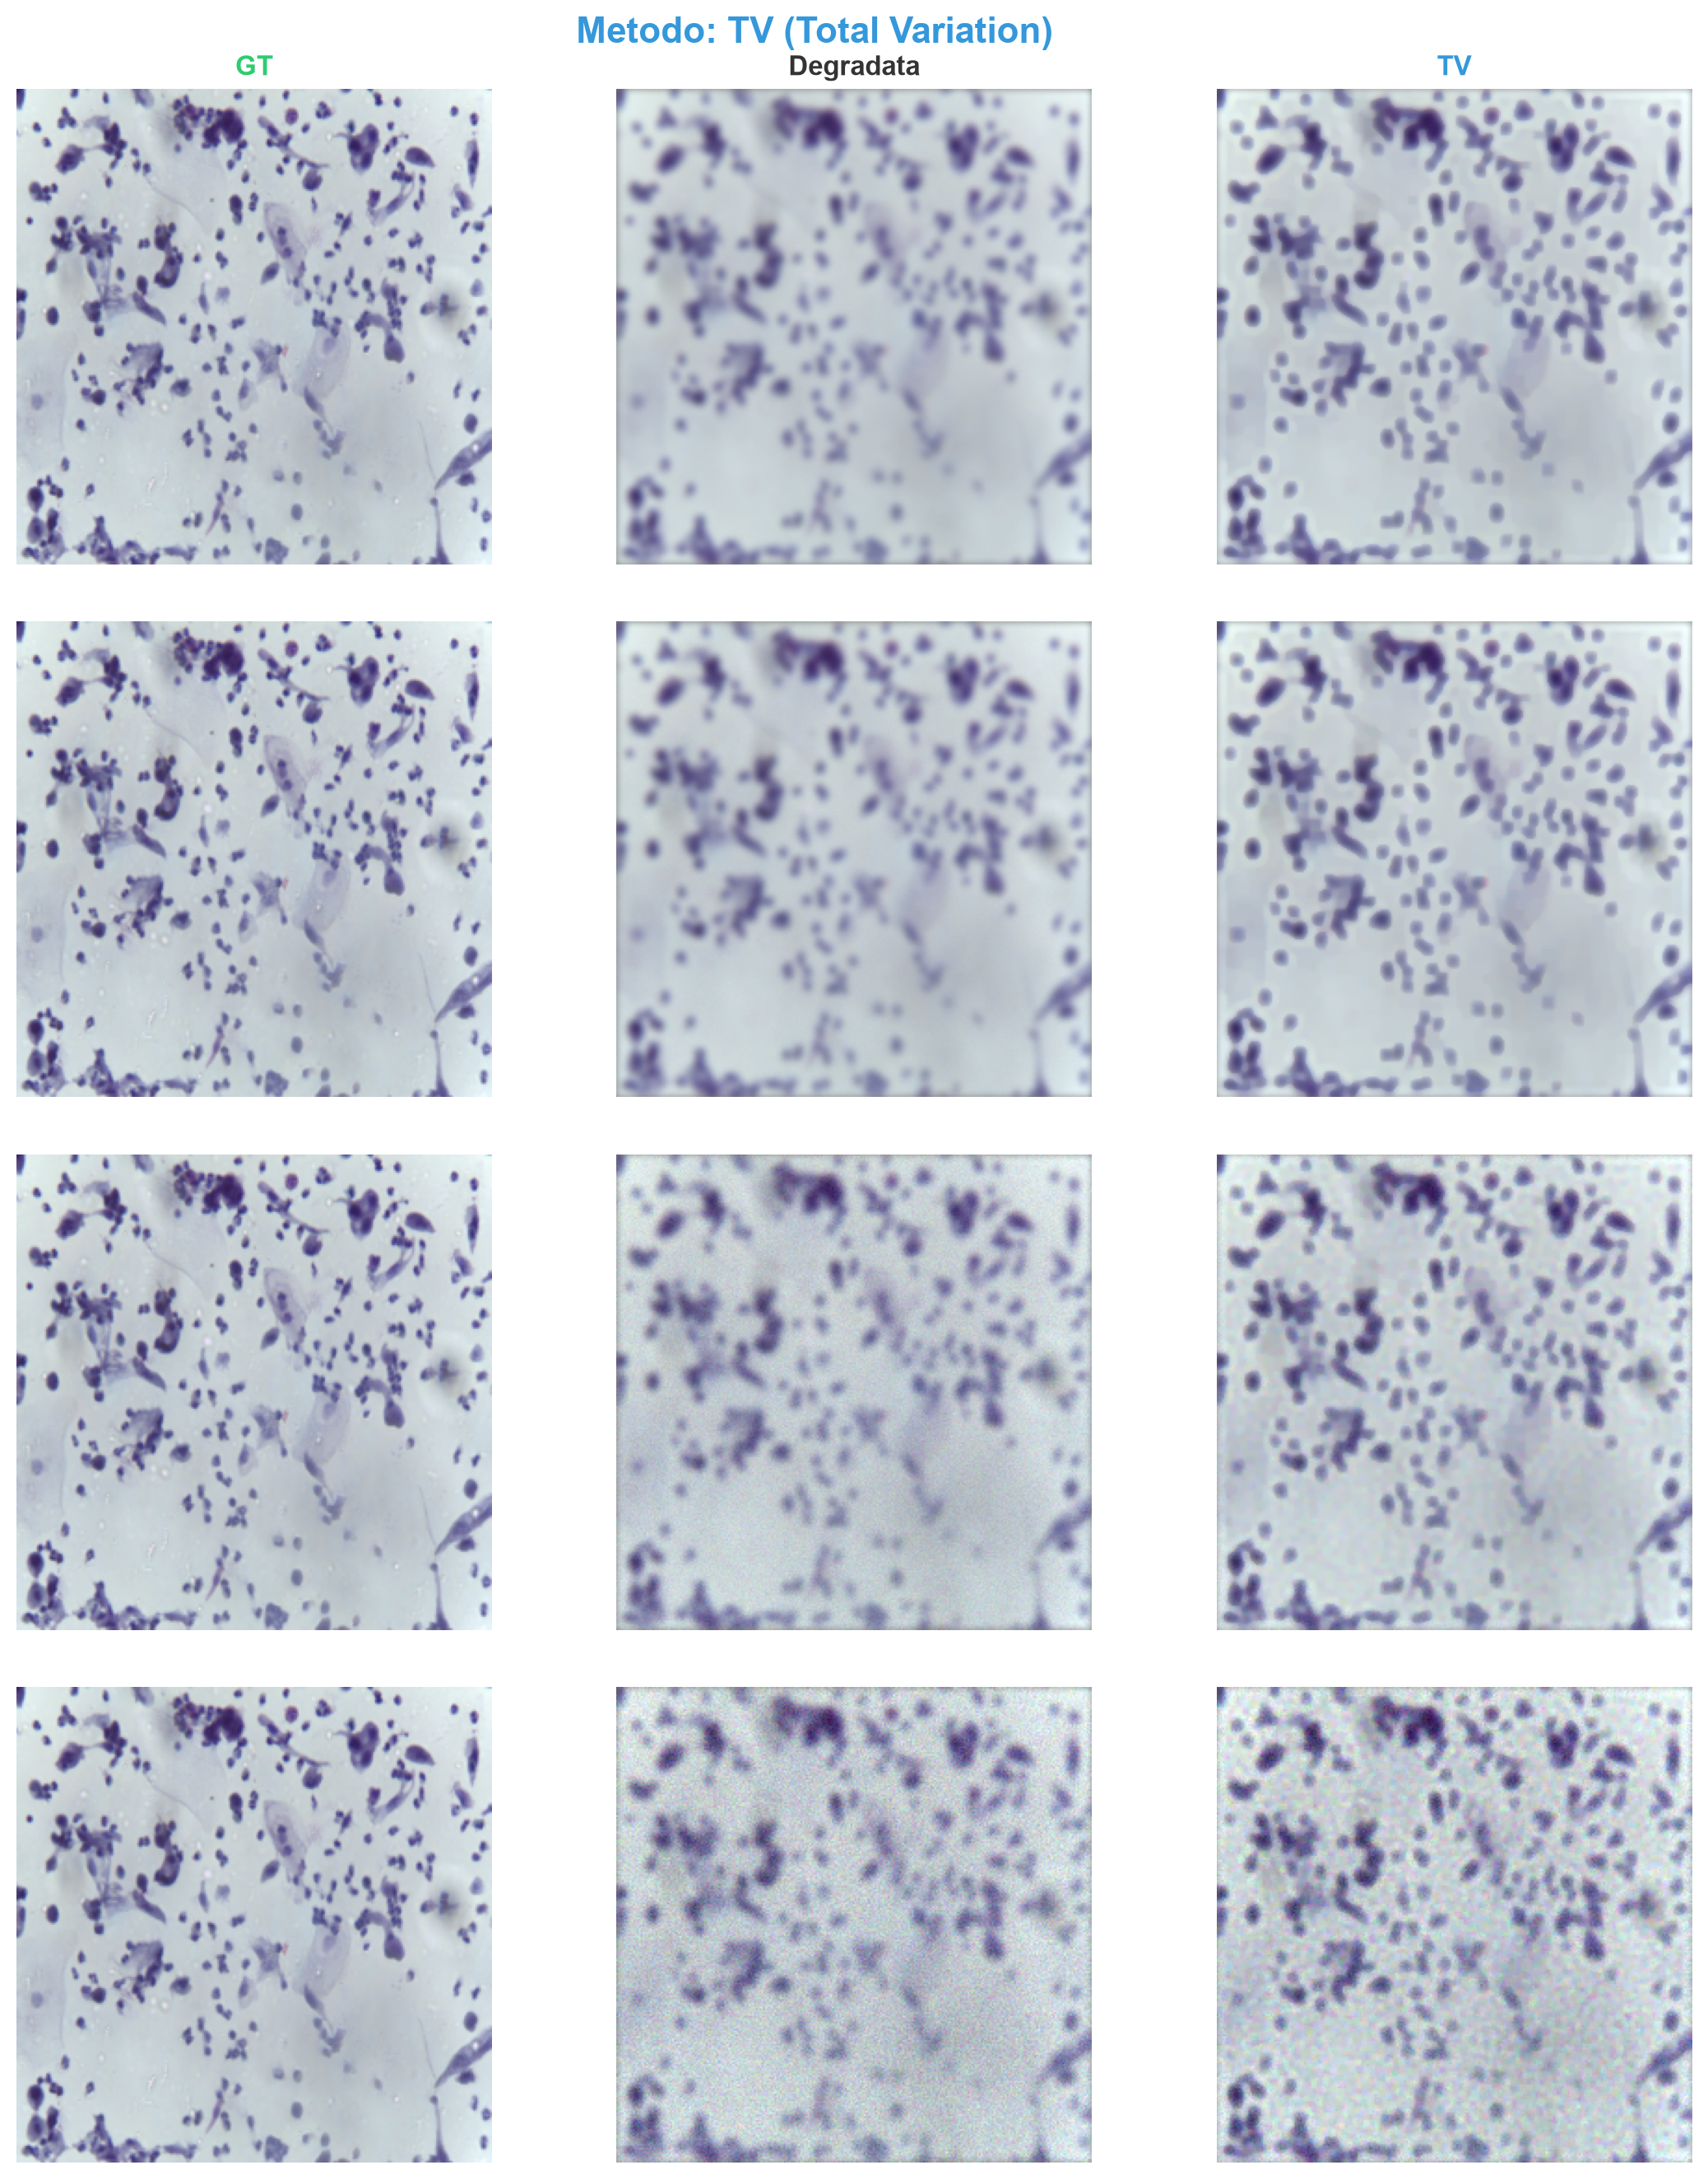
\includegraphics[width=\textwidth]{../results/qualitative_slides/tv_comparison.png}
  \end{columns}
\end{frame}

\section{UNet -- Paolo}

\begin{frame}{UNet -- Architettura}
  \begin{block}{Encoder-Decoder con Skip Connections}
    Architettura snella per image-to-image: degradata $\to$ restaurata
  \end{block}
  \vspace{0.2cm}
  \begin{center}
    \begin{tikzpicture}[scale=0.42, every node/.style={scale=0.8,font=\ttfamily\bfseries}]
      \fill[gray!20] (0,0) rectangle (2,2);
      \fill[gray!30] (2.5,0) rectangle (4.5,2);
      \fill[gray!40] (5,0) rectangle (7,2);
      \fill[gray!50] (7.5,0) rectangle (9.5,2);
      \fill[gray!60] (10,0) rectangle (12,2);
      \fill[gray!50] (12.5,3.5) rectangle (14.5,5.5);
      \fill[gray!40] (15,3.5) rectangle (17,5.5);
      \fill[gray!30] (17.5,3.5) rectangle (19.5,5.5);
      \fill[gray!20] (20,3.5) rectangle (22,5.5);
      \draw (1,1) node {16};
      \draw (3.5,1) node {32};
      \draw (6,1) node {64};
      \draw (8.5,1) node {128};
      \draw (11,1) node {256};
      \draw (13.5,4.5) node {128};
      \draw (16,4.5) node {64};
      \draw (18.5,4.5) node {32};
      \draw (21,4.5) node {16};
      \draw[->,thick] (2.2,1) -- (2.3,1);
      \draw[->,thick] (4.7,1) -- (4.8,1);
      \draw[->,thick] (7.2,1) -- (7.3,1);
      \draw[->,thick] (9.7,1) -- (9.8,1);
      \draw[->,thick] (12.2,2.2) -- (12.2,3.3);
      \draw[->,thick] (14.7,4.5) -- (14.8,4.5);
      \draw[->,thick] (17.2,4.5) -- (17.3,4.5);
      \draw[->,thick] (19.7,4.5) -- (19.8,4.5);
      \draw[dashed,gray,->] (2,0.5) to[out=60,in=180] (22,0.5);
    \end{tikzpicture}
  \end{center}
  \vspace{0.3cm}
  \hfill\small (skip connections: encoder $\to$ decoder allo stesso livello)
  \vspace{0.2cm}
  \begin{columns}
    \column{0.5\textwidth}
      \begin{itemize}
        \item Canali: 16 $\to$ 32 $\to$ 64 $\to$ 128 $\to$ 256
        \item Blocco: DoubleConv (Conv3$\times$3, GroupNorm, ReLU)
      \end{itemize}
    \column{0.5\textwidth}
      \begin{itemize}
        \item Input: RGB + noise map (4 canali)
        \item Output: RGB + $\tanh$ (range $[-1,1]$)
        \item $\sim$1.9M parametri
      \end{itemize}
  \end{columns}
\end{frame}

\begin{frame}{UNet -- Training}
  \begin{columns}
    \column{0.48\textwidth}
      \begin{block}{Configurazione}
        \begin{tabular}{ll}\toprule
          \textbf{Parametro} & \textbf{Valore}\\\midrule
          Loss & L1 (MAE)\\
          Ottimizzatore & Adam\\
          Learning rate & $10^{-4}$\\
          Batch size & 16\\
          Epoche & 50\\
          Noise aug. & Uniforme $\sigma_n$\\\bottomrule
        \end{tabular}
      \end{block}
      \vspace{0.2cm}
      \textbf{Multi-noise augmentation:}
      $\sigma_n$ random per batch
      \begin{itemize}
        \item Modello robusto su tutti i livelli
        \item Evita overfitting su un singolo $\sigma_n$
      \end{itemize}
    \column{0.52\textwidth}
      \small
      \textbf{Pseudo-codice training:}
      \vspace{0.15cm}
      \begin{enumerate}
        \item \textbf{for} epoch $=1$ \textbf{to} $50$ \textbf{do}
        \item \hspace{0.5cm}\textbf{for} batch $b$ \textbf{in} train\_loader \textbf{do}
        \item \hspace{1.0cm}$\sigma \gets \text{Uniform}\{\sigma_n\}$
        \item \hspace{1.0cm}$\tilde{b} \gets \text{degrade}(b, \sigma)$
        \item \hspace{1.0cm}$\hat{b} \gets \text{UNet}(\tilde{b})$ \hfill\tiny forward
        \item \hspace{1.0cm}$\mathcal{L} \gets \|\hat{b} - b\|_1$ \hfill\tiny L1 loss
        \item \hspace{1.0cm}$\nabla_\theta\mathcal{L} \gets$ backprop \hfill\tiny backward
        \item \hspace{1.0cm}$\theta \gets$ AdamStep$(\theta)$ \hfill\tiny update
        \item \hspace{0.5cm}\textbf{end for}
        \item \hspace{0.5cm}val\_psnr $\gets$ validate(model)
        \item \hspace{0.5cm}save if val\_psnr $>$ best
        \item \textbf{end for}
      \end{enumerate}
      \vspace{0.2cm}
      \small
      \textbf{Checkpoint:} \texttt{results/unet/best\_model.pth}
  \end{columns}
\end{frame}

\begin{frame}{UNet -- Risultati}
  \begin{columns}
    \column{0.5\textwidth}
      \textbf{PSNR e SSIM su 145 immagini test}
      \vspace{0.2cm}
      \begin{tabular}{l|ccc}\toprule
        $\sigma_n$ & \textbf{PSNR} & \textbf{SSIM} & \textbf{Tempo}\\\midrule
         0.005 & 29.79 & 0.896 & 0.030 s\\
         0.01  & 29.79 & 0.895 & 0.028 s\\
         0.05  & 29.44 & 0.864 & 0.027 s\\
         0.1   & 28.46 & 0.795 & 0.026 s\\\bottomrule
      \end{tabular}
      \vspace{0.3cm}
      \begin{itemize}
        \item Degradazione minima ($\sim$1 dB tra estremi)
        \item \textbf{Supera TV} a $\sigma_n=0.1$ (28.46 vs 26.54 dB)
        \item Inferenza pi\`u veloce: 0.035 s/img
      \end{itemize}
    \column{0.5\textwidth}
      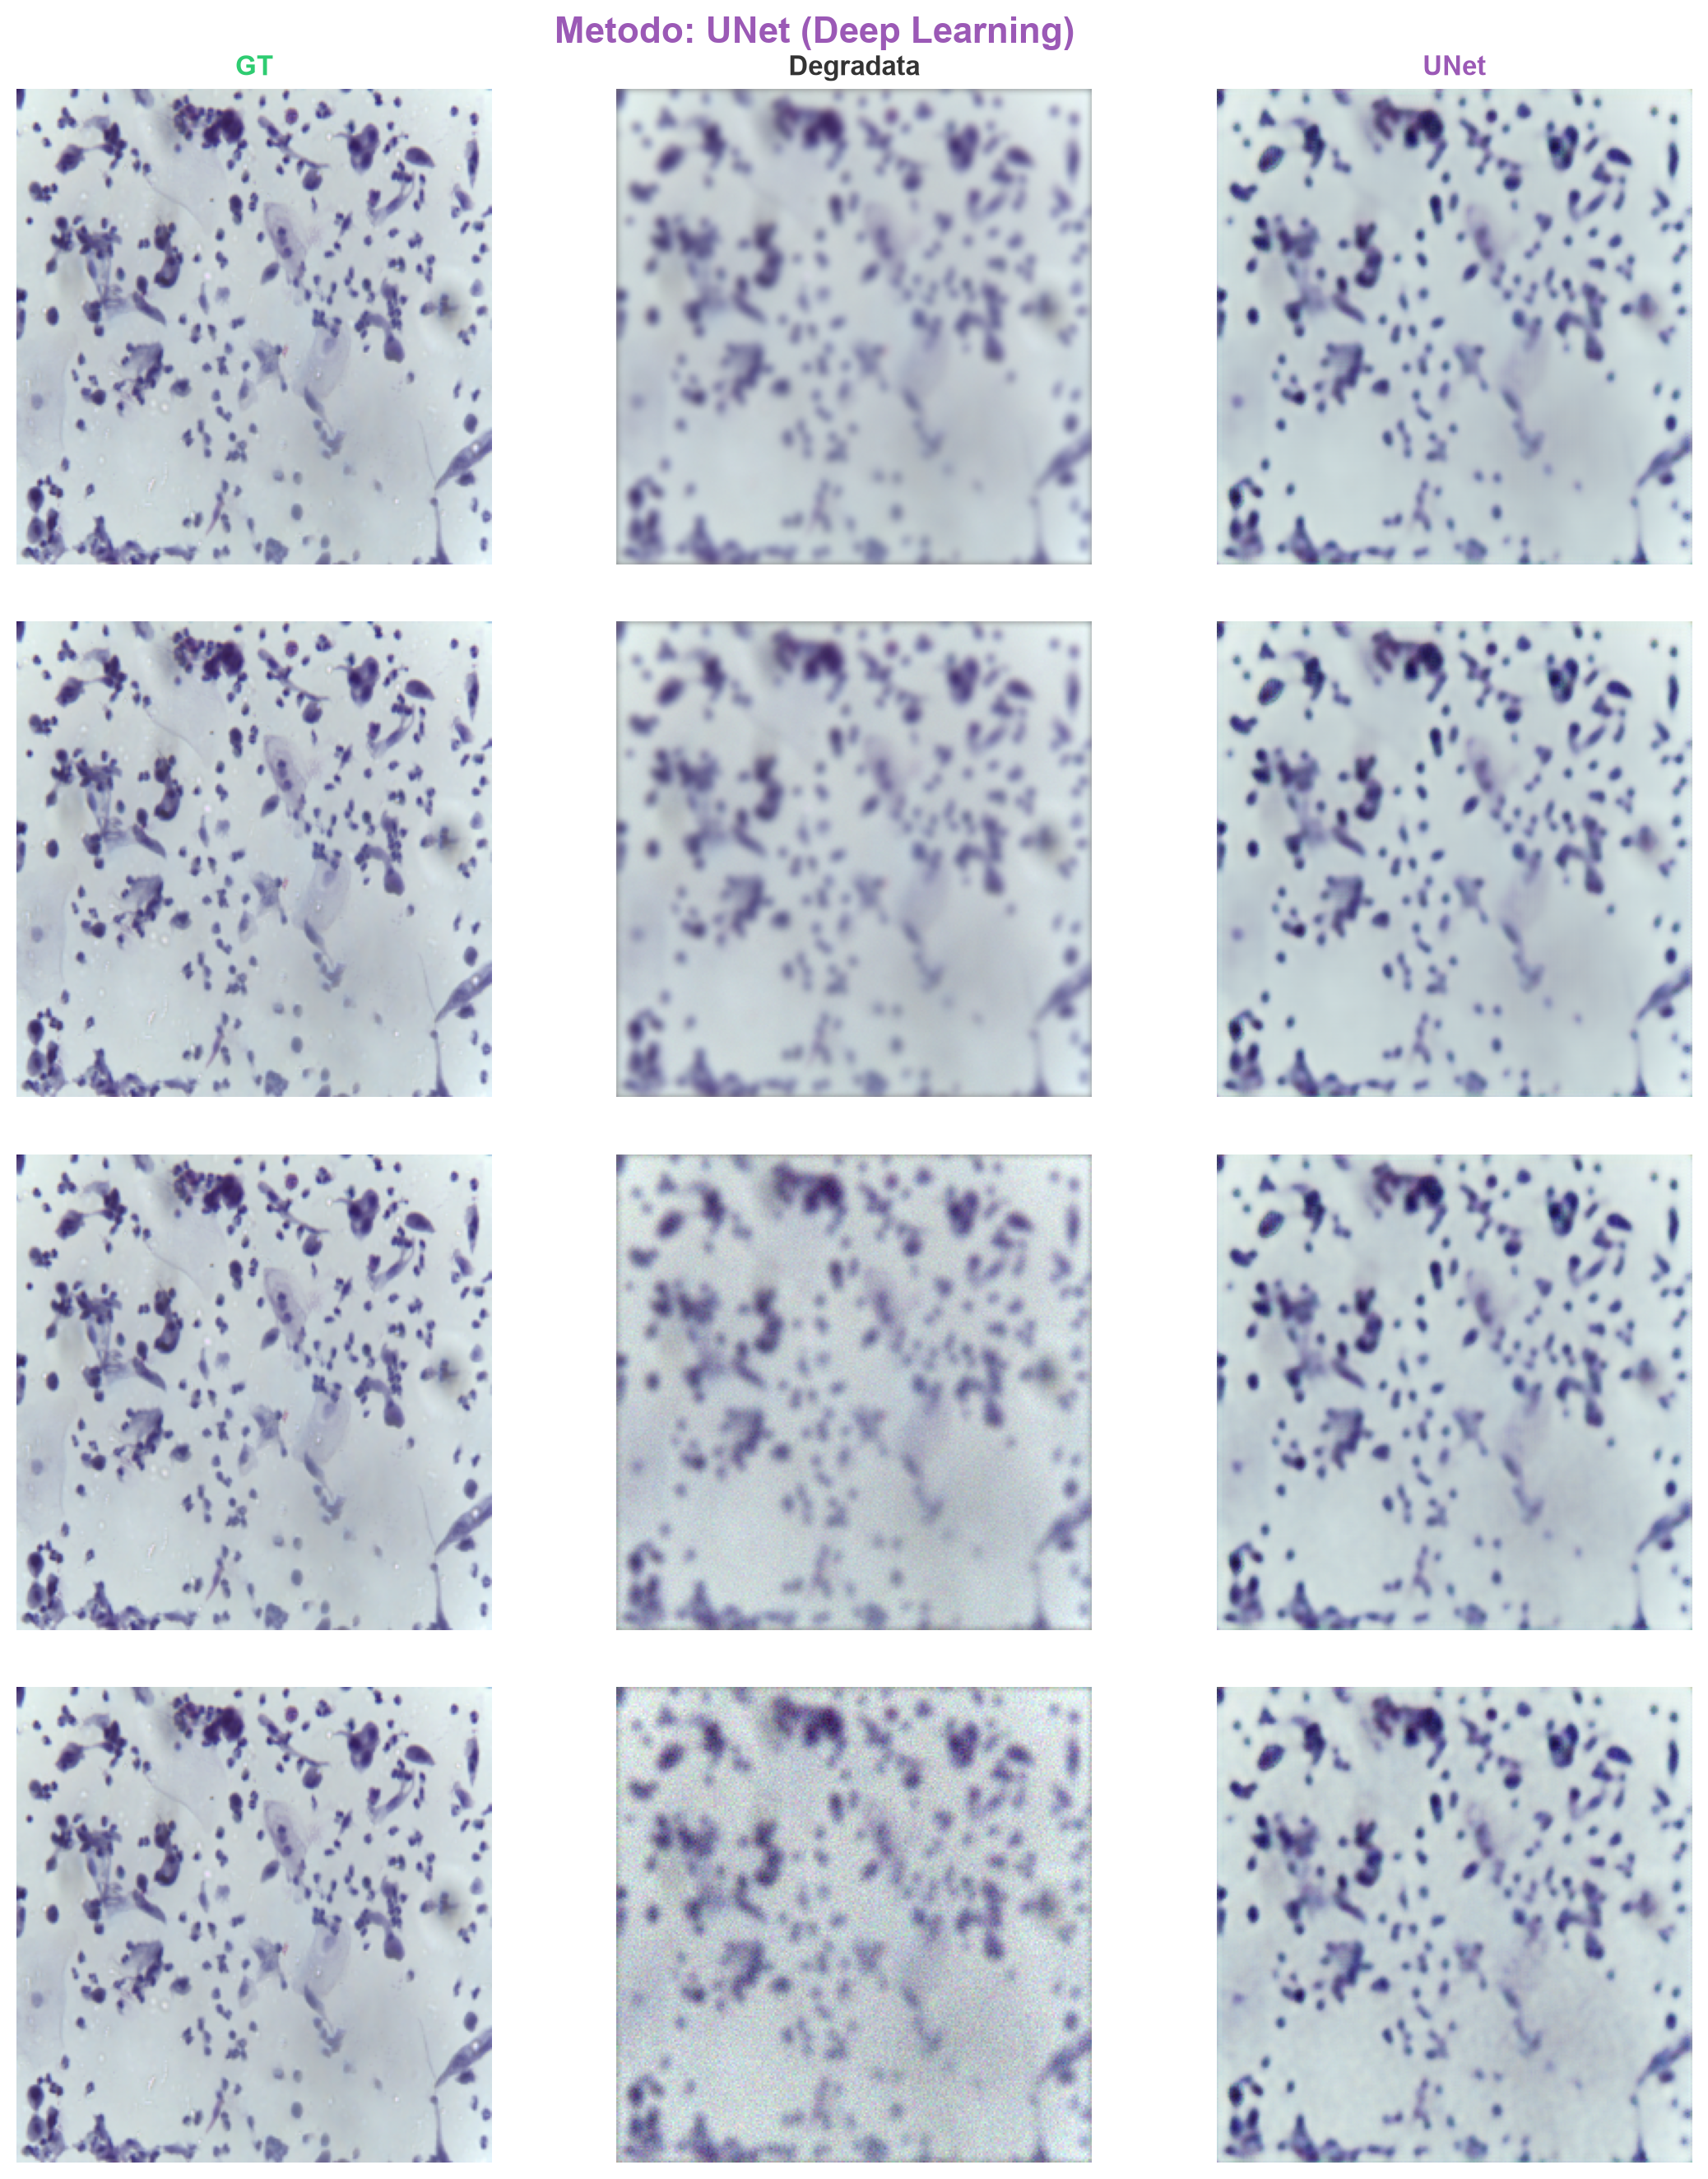
\includegraphics[width=\textwidth]{../results/qualitative_slides/unet_comparison.png}
  \end{columns}
\end{frame}

\section{DiffPIR -- Francesco}

\begin{frame}{DiffPIR -- Panoramica}
  \begin{block}{DiffPIR (Diffusion-based Plug-and-Play Image Restoration)}
    \begin{itemize}
      \item Integra un \textbf{modello di diffusione} (DDPM) in framework Plug-and-Play
      \item Alterna \textbf{denoising} (prior generativo) e \textbf{data-fidelity} (via FFT)
    \end{itemize}
  \end{block}
  \begin{alertblock}{LightUNet custom (1.26M params, $\sim$5 MB)}
    Addestrata da zero su 673 immagini LBC cervicali\\[0.1cm]
    $\triangleright$ Specifica per il dominio citologico \\[0.1cm]
    $\triangleright$ Training e inferenza su CPU
  \end{alertblock}
\end{frame}

\begin{frame}{DDPM e LightUNet}
  \begin{columns}
    \column{0.55\textwidth}
      \textbf{Denoising Diffusion Probabilistic Models}
      \begin{itemize}\small
        \item 1000 timestep, $\beta_1=10^{-4}$, $\beta_T=0.02$
        \item Loss: MSE su $\varepsilon_\theta(x_t,t)$
        \item Training: 673 immagini, 30 epoche
      \end{itemize}
      \vspace{0.2cm}
      \textbf{LightUNet}
      \begin{itemize}\small
        \item Canali base: 32
        \item Encoder: 32$\to$64$\to$128
        \item Time embedding sinusoidale + MLP
        \item GroupNorm + SiLU
        \item \textbf{1,262,273 parametri}
      \end{itemize}
    \column{0.45\textwidth}
      \begin{block}{Processo di Diffusione}
        \centering\small
        $x_0 \to x_1 \to \cdots \to x_T$ \\[0.1cm]
        \textbf{Forward} \\
        $q(x_t|x_{t-1}) = \mathcal{N}(\sqrt{1-\beta_t}x_{t-1}, \beta_t I)$ \\[0.2cm]
        \textbf{Reverse} \\
        $p_\theta(x_{t-1}|x_t) = \mathcal{N}(\mu_\theta(x_t,t), \Sigma_\theta(x_t,t))$
      \end{block}
  \end{columns}
\end{frame}

\begin{frame}{Algoritmo DiffPIR}
  \begin{columns}
    \column{0.55\textwidth}
      \small
      \textbf{Pseudo-codice:}
      \vspace{0.1cm}
      \begin{enumerate}
        \item $y \gets$ immagine degradata
        \item $\mathcal{K} \gets \text{FFT}(k)$ \hfill\tiny kernel OTF
        \item \textbf{for} $t = t_{\text{start}}$ \textbf{to} $1$ \textbf{do}
        \item \hspace{0.5cm}$\varepsilon \gets \varepsilon_\theta(x_t, t)$ \hfill\tiny DDPM denoise
        \item \hspace{0.5cm}$\hat{x}_0 \gets \frac{x_t - \sqrt{1-\bar{\alpha}_t}\,\varepsilon}{\sqrt{\bar{\alpha}_t}}$
        \item \hspace{0.5cm}$\hat{x}_0 \gets \text{clamp}(\hat{x}_0, -1, 1)$
        \item \hspace{0.5cm}$\rho_t \gets \lambda \cdot \frac{\sigma^2 \bar{\alpha}_t}{1 - \bar{\alpha}_t}$
        \item \hspace{0.5cm}$\tilde{x}_0 \gets \mathcal{F}^{-1}\!\left(\frac{\mathcal{F}(y)\overline{\mathcal{K}} + \rho_t\mathcal{F}(\hat{x}_0)}{|\mathcal{K}|^2 + \rho_t}\right)$
        \item \hspace{0.5cm}$x_{t-1} \gets$ DDIM step$(x_t, \tilde{x}_0)$
        \item \textbf{end for}
        \item \textbf{return} $x_0$
      \end{enumerate}
    \column{0.45\textwidth}
      \small
      \textbf{Step 1 -- Denoising:}
      \begin{equation*}
        \hat{x}_0^{(t)} = \frac{x_t - \sqrt{1-\bar{\alpha}_t}\,\varepsilon_\theta(x_t,t)}{\sqrt{\bar{\alpha}_t}}
      \end{equation*}
      \vspace{0.15cm}
      \textbf{Step 2 -- Data Fidelity (FFT):}
      \begin{equation*}
        \tilde{x}_0 = \mathcal{F}^{-1}\!\left(
        \frac{\mathcal{F}(y)\overline{\mathcal{F}(k)} + \rho\mathcal{F}(\hat{x}_0)}
             {|\mathcal{F}(k)|^2 + \rho}\right)
      \end{equation*}
      \vspace{0.15cm}
      \textbf{Peso dinamico:}
      \begin{equation*}
        \rho_t = \lambda \cdot \frac{\sigma^2 \cdot \bar{\alpha}_t}{1 - \bar{\alpha}_t}
      \end{equation*}
  \end{columns}
\end{frame}

\begin{frame}{DiffPIR -- Parametri e Risultati}
  \begin{columns}
    \column{0.45\textwidth}
      \textbf{Scelta euristica dei parametri}
      \begin{tabular}{ll}\toprule
        \textbf{Parametro} & \textbf{Valore}\\\midrule
        $t_{\text{start}}$ & 50\\
        $\lambda$ & 10.0\\
        $num\_steps$ & 15\\
        $\zeta$ & 0.0 (DDIM)\\\bottomrule
      \end{tabular}
      \vspace{0.3cm}
      \textbf{Risultati quantitativi}
      \begin{tabular}{l|cc}\toprule
        $\sigma_n$ & \textbf{PSNR} & \textbf{SSIM}\\\midrule
        0.005 & 15.78 & 0.329\\
        0.01  & 16.45 & 0.374\\
        0.05  & 22.64 & 0.677\\
        0.1   & 25.46 & 0.766\\\bottomrule
      \end{tabular}
      \vspace{0.2cm}
      \begin{itemize}
        \item PSNR \textbf{cresce} col rumore
        \item Migliore a $\sigma_n=0.1$ (25.46 dB)
      \end{itemize}
    \column{0.55\textwidth}
      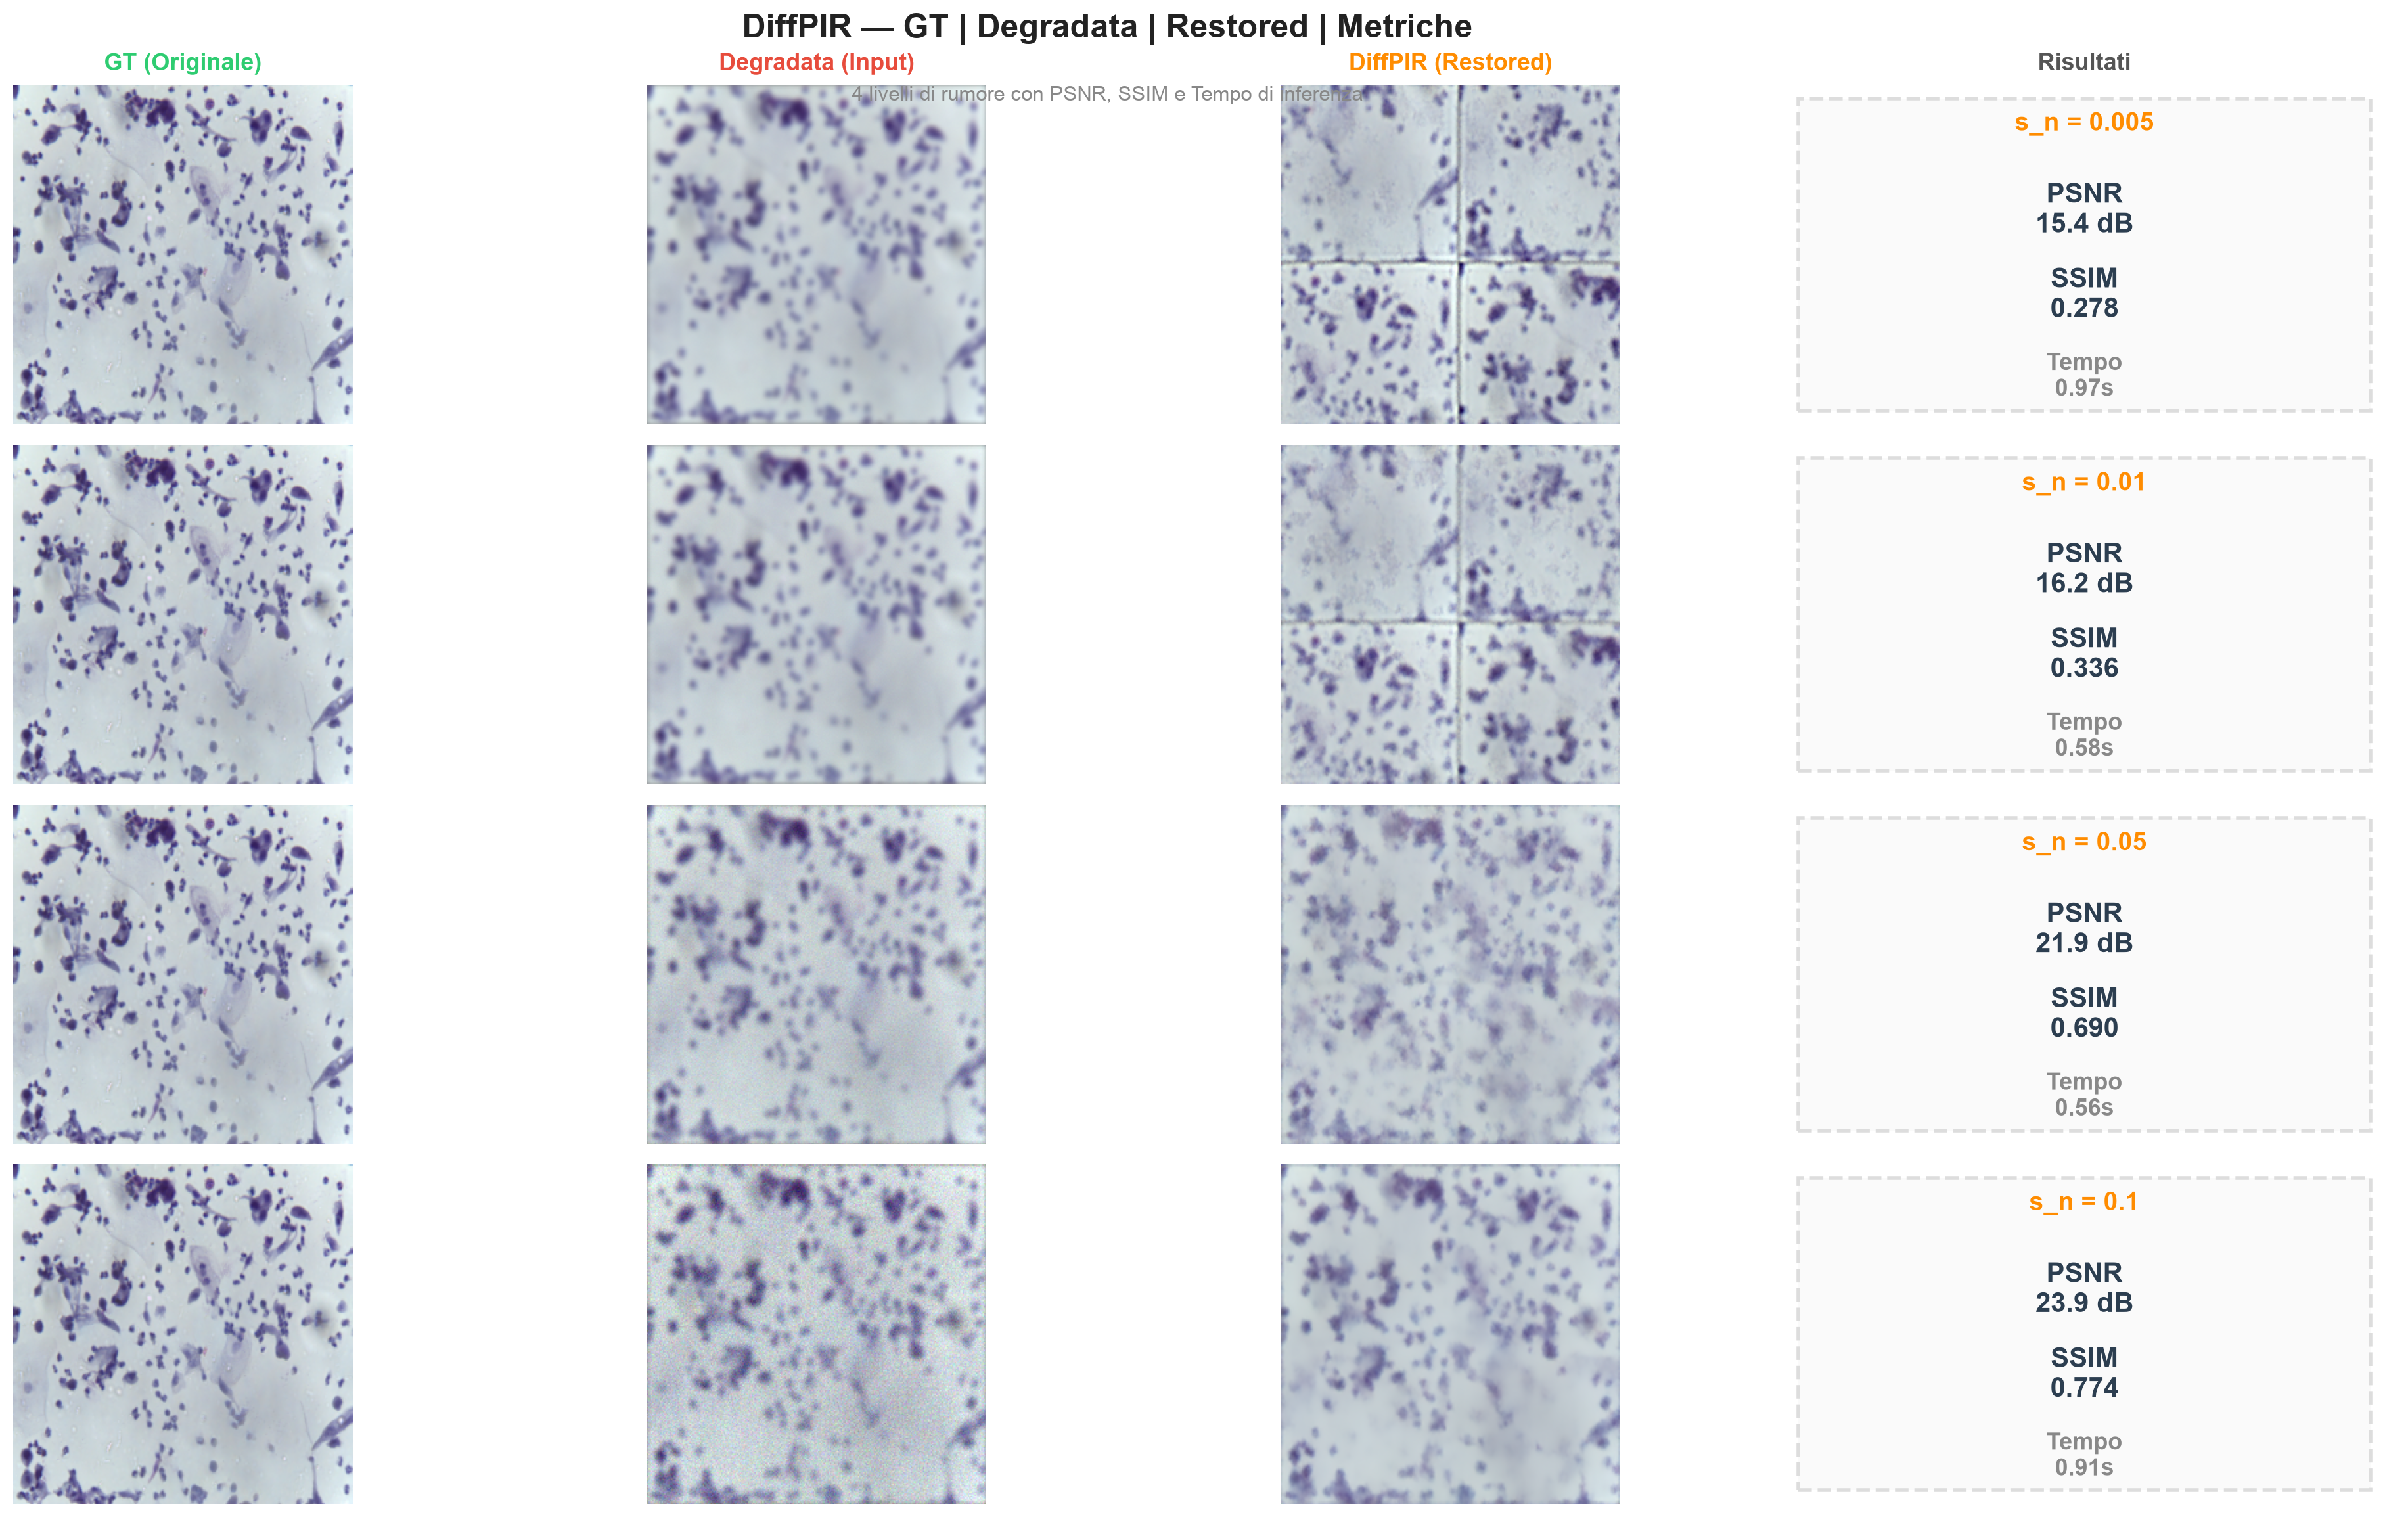
\includegraphics[width=\textwidth]{../results/qualitative_slides/diffpir_2x4.png}
  \end{columns}
\end{frame}

\section{Implementazione}

\begin{frame}{Implementazione -- Struttura del Repository}
  \begin{columns}
    \column{0.55\textwidth}
      \textbf{Albero del progetto}
      \vspace{0.1cm}
      \begin{center}
      \begin{tikzpicture}[scale=0.42, every node/.style={font=\scriptsize\ttfamily}]
        \node[anchor=west] at (0,0) {ci-cervical-lbc/};
        \node[anchor=west] at (0.6,-0.6) {src/};
        \node[anchor=west] at (1.2,-1.2) {data/dataset.py};
        \node[anchor=west] at (1.2,-1.8) {degradation/degradation.py};
        \node[anchor=west] at (1.2,-2.4) {methods/};
        \node[anchor=west] at (1.8,-3.0) {tv/tv.py};
        \node[anchor=west] at (1.8,-3.6) {unet/unet.py};
        \node[anchor=west] at (1.8,-4.2) {diffpir/};
        \node[anchor=west] at (2.4,-4.8) {diffpir.py, model.py, train.py};
        \node[anchor=west] at (0.6,-5.4) {scripts/ (run\_tv.py, run\_unet.py, run\_diffpir.py)};
        \node[anchor=west] at (0.6,-6.0) {tests/ (34 unit test)};
        \node[anchor=west] at (0.6,-6.6) {results/ (tv/, unet/, diffpir/)};
        \node[anchor=west] at (0.6,-7.2) {configs/experiment.yaml};
      \end{tikzpicture}
      \end{center}
    \column{0.45\textwidth}
      \textbf{Modularità}
      \begin{itemize}
        \item Ogni metodo è un modulo indipendente
        \item Pipeline condivisa: degradazione, metriche
        \item Stesso test set per tutti
      \end{itemize}
      \vspace{0.3cm}
      \textbf{Esecuzione:}
      \vspace{0.1cm}
      \begin{enumerate}
        \item \texttt{python scripts/preprocess.py}
        \item \texttt{python scripts/run\_tv.py}
        \item \texttt{python scripts/run\_unet.py}
        \item \texttt{python scripts/run\_diffpir.py}
        \item \texttt{python scripts/plot\_results.py}
      \end{enumerate}
      \vspace{0.3cm}
      \begin{block}{Riproducibilità}
        Seed 42, pipeline unica, 34 unit test
      \end{block}
  \end{columns}
\end{frame}

\section{Risultati Quantitativi}

\begin{frame}{Confronto PSNR / SSIM}
  \small
  \begin{tabular}{l|ccc|ccc}\toprule
    & \multicolumn{3}{c|}{\textbf{PSNR (dB) $\uparrow$}} & \multicolumn{3}{c}{\textbf{SSIM $\uparrow$}}\\
    $\sigma_n$ & \textbf{TV} & \textbf{UNet} & \textbf{DiffPIR} & \textbf{TV} & \textbf{UNet} & \textbf{DiffPIR}\\\midrule
     0.005 & \textbf{32.09} & 29.79 & 15.78 & \textbf{0.911} & 0.896 & 0.329\\
     0.01  & \textbf{32.04} & 29.79 & 16.45 & \textbf{0.909} & 0.895 & 0.374\\
     0.05  & \textbf{30.42} & 29.44 & 22.64 & 0.837 & \textbf{0.864} & 0.677\\
     0.1   & 26.54 & \textbf{28.46} & 25.46 & 0.586 & \textbf{0.795} & 0.766\\\bottomrule
  \end{tabular}
  \vspace{0.3cm}
  \begin{block}{Osservazioni}
    \begin{itemize}
      \item \textbf{TV}: domina a $\sigma_n\leq0.01$ (PSNR $>$ 32 dB, SSIM $>$ 0.9)
      \item \textbf{UNet}: miglior compromesso, degradazione $\sim$1 dB, supera TV a $\sigma_n=0.1$
      \item \textbf{DiffPIR}: generativo, PSNR cresce col rumore (15.78$\to$25.46 dB)
    \end{itemize}
  \end{block}
\end{frame}

\begin{frame}{Grafico Comparativo}
  \begin{center}
    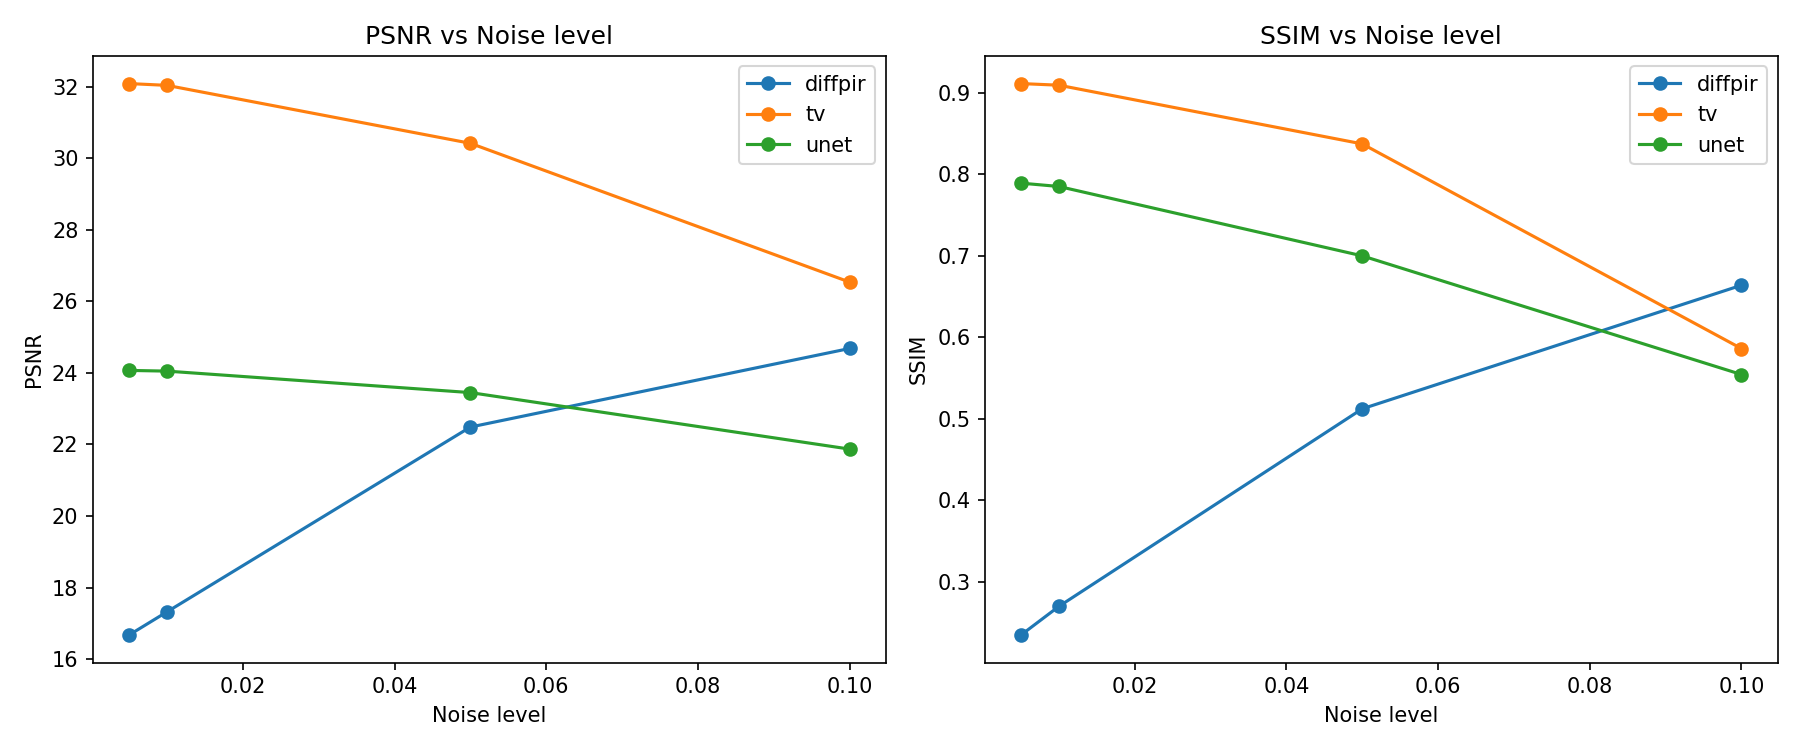
\includegraphics[width=0.92\textwidth]{../results/comparison.png}
  \end{center}
\end{frame}

\section{Risultati Qualitativi}

\begin{frame}{Griglia Completa}
  \begin{center}
    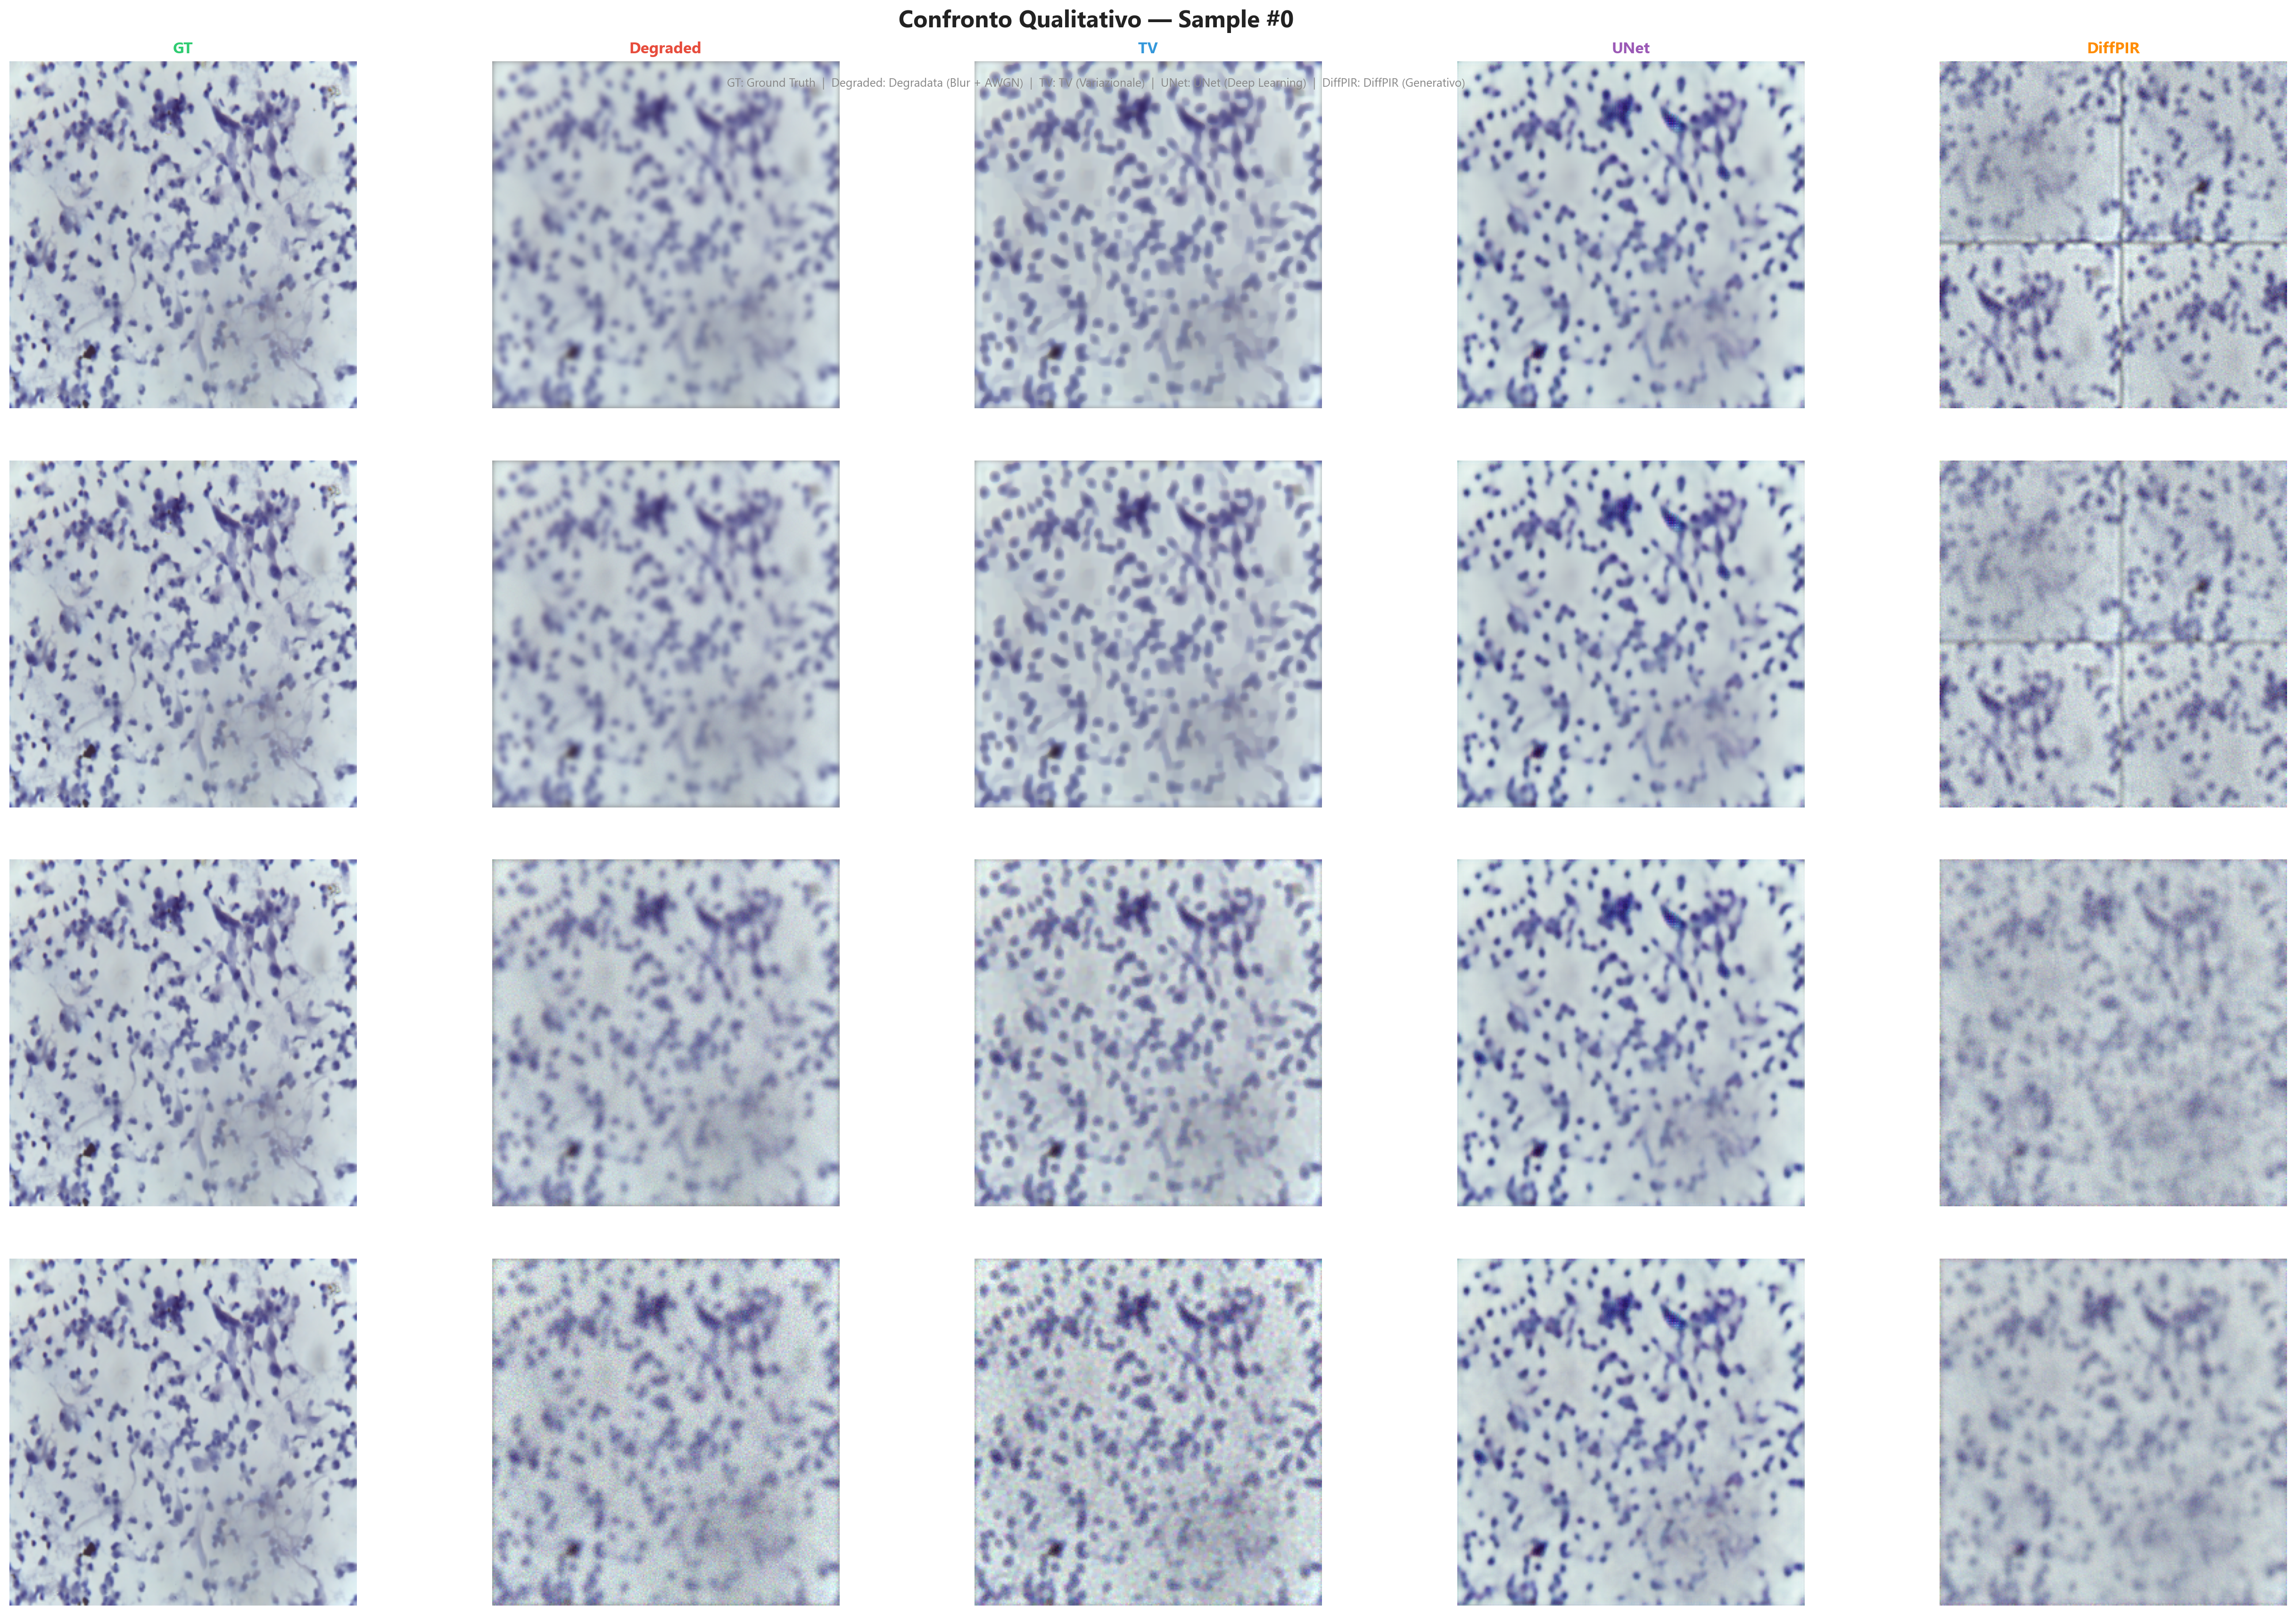
\includegraphics[width=0.7\textwidth]{../results/qualitative_slides/all_methods_grid.png}
  \end{center}
\end{frame}

\begin{frame}{Confronto Visivo -- $\sigma_n = 0.01$}
  \begin{center}
    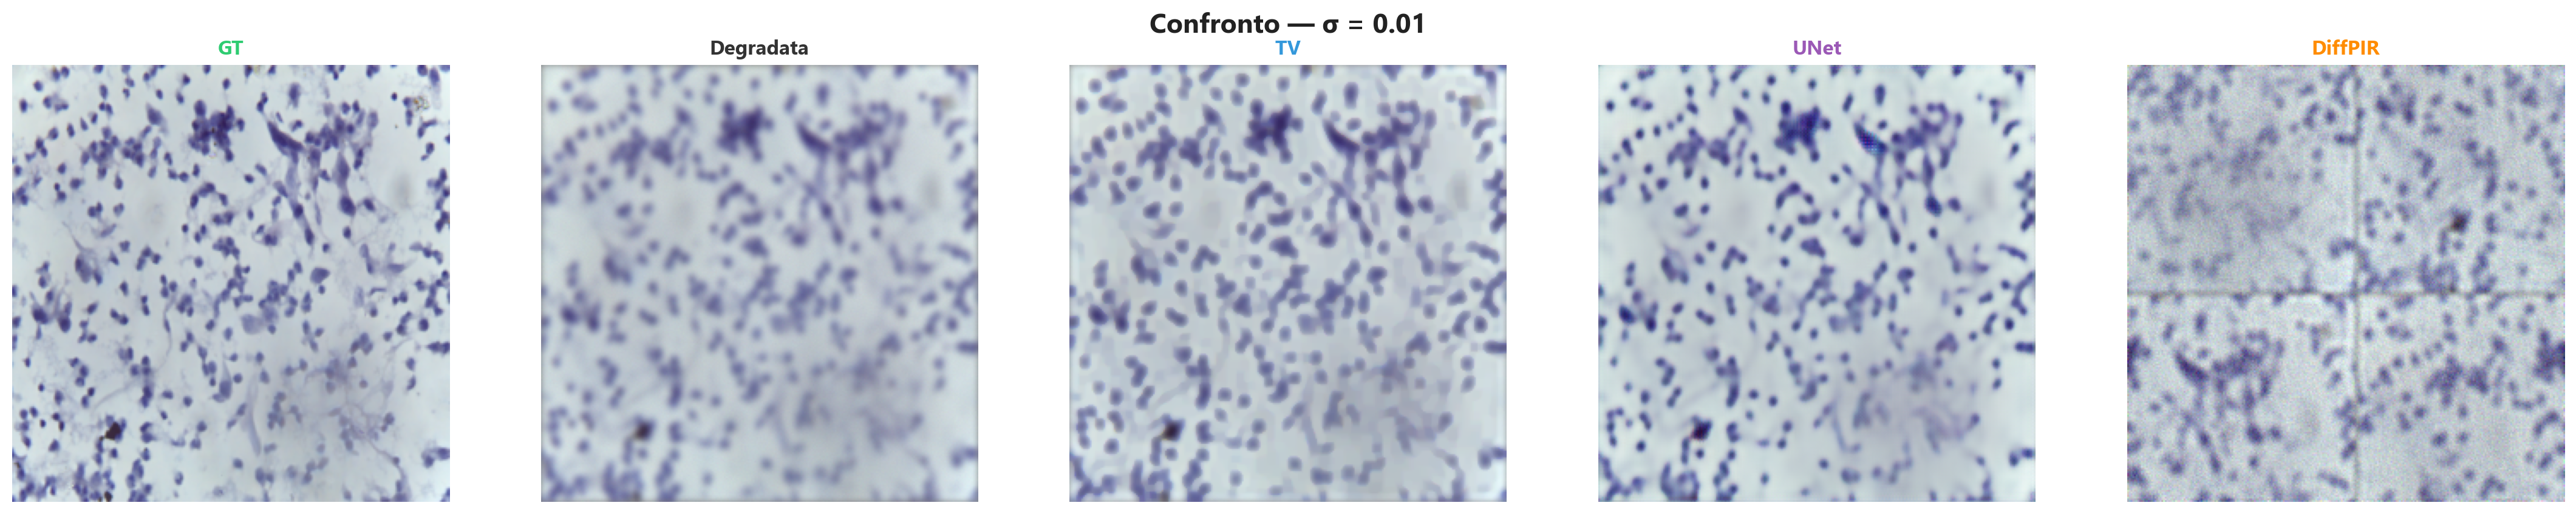
\includegraphics[width=0.95\textwidth]{../results/qualitative_slides/noise_0.01_comparison.png}
    \vspace{0.3cm}
    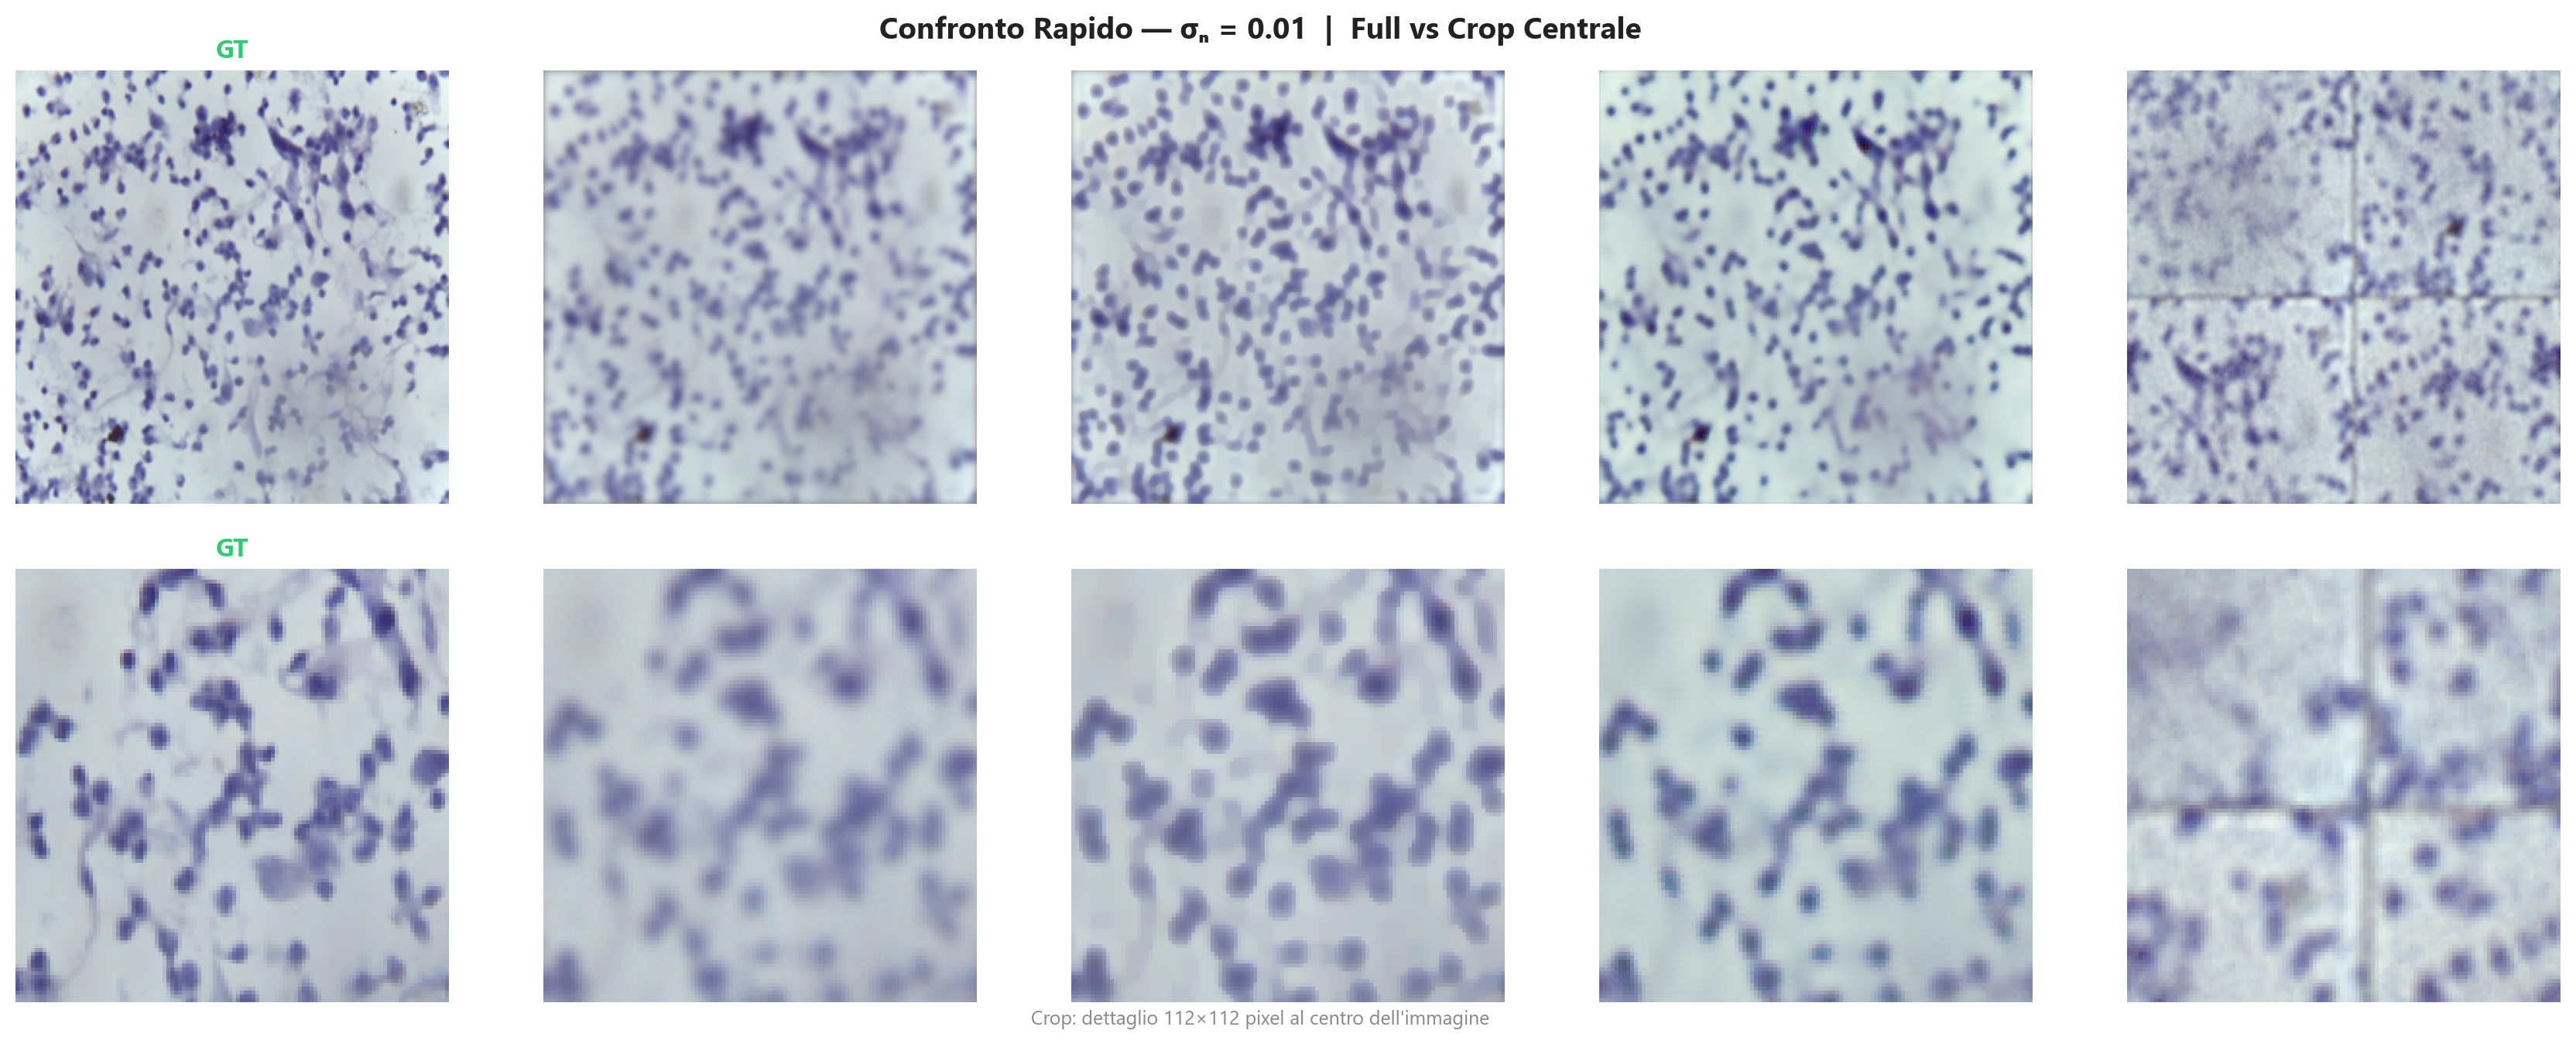
\includegraphics[width=0.74\textwidth]{../results/qualitative_slides/crop_comparison.png}
  \end{center}
\end{frame}

\begin{frame}{Confronto Visivo -- $\sigma_n = 0.05$}
  \begin{center}
    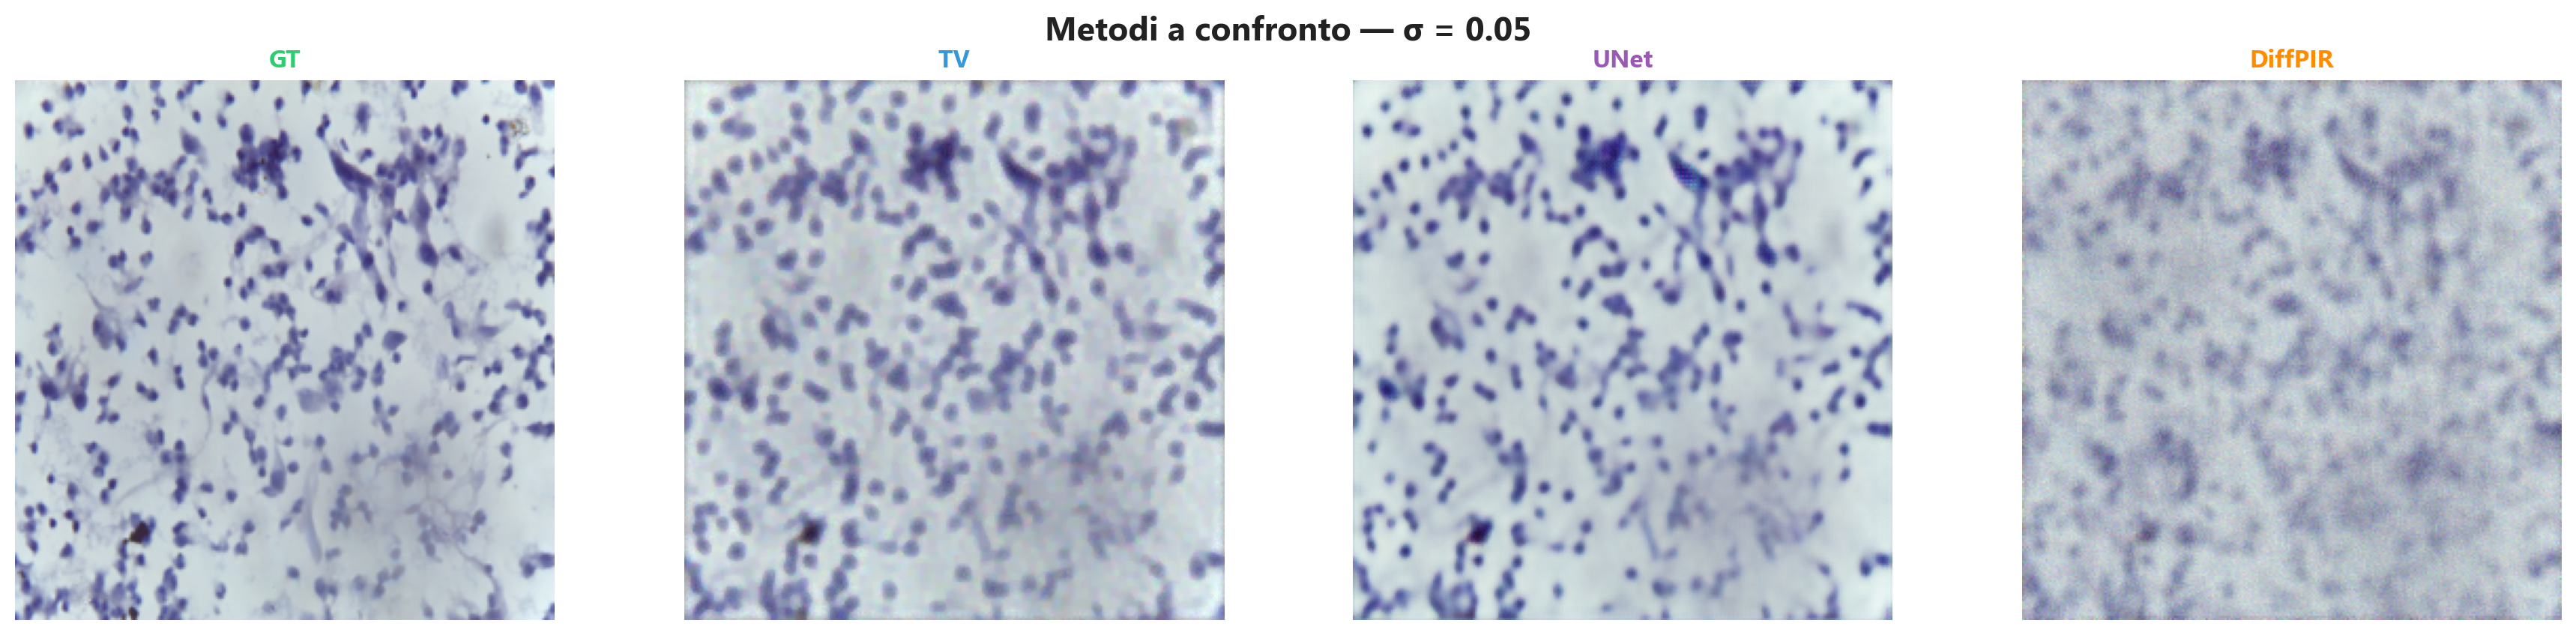
\includegraphics[width=0.95\textwidth]{../results/qualitative_slides/methods_noise_0.05.png}
    \vspace{0.3cm}
    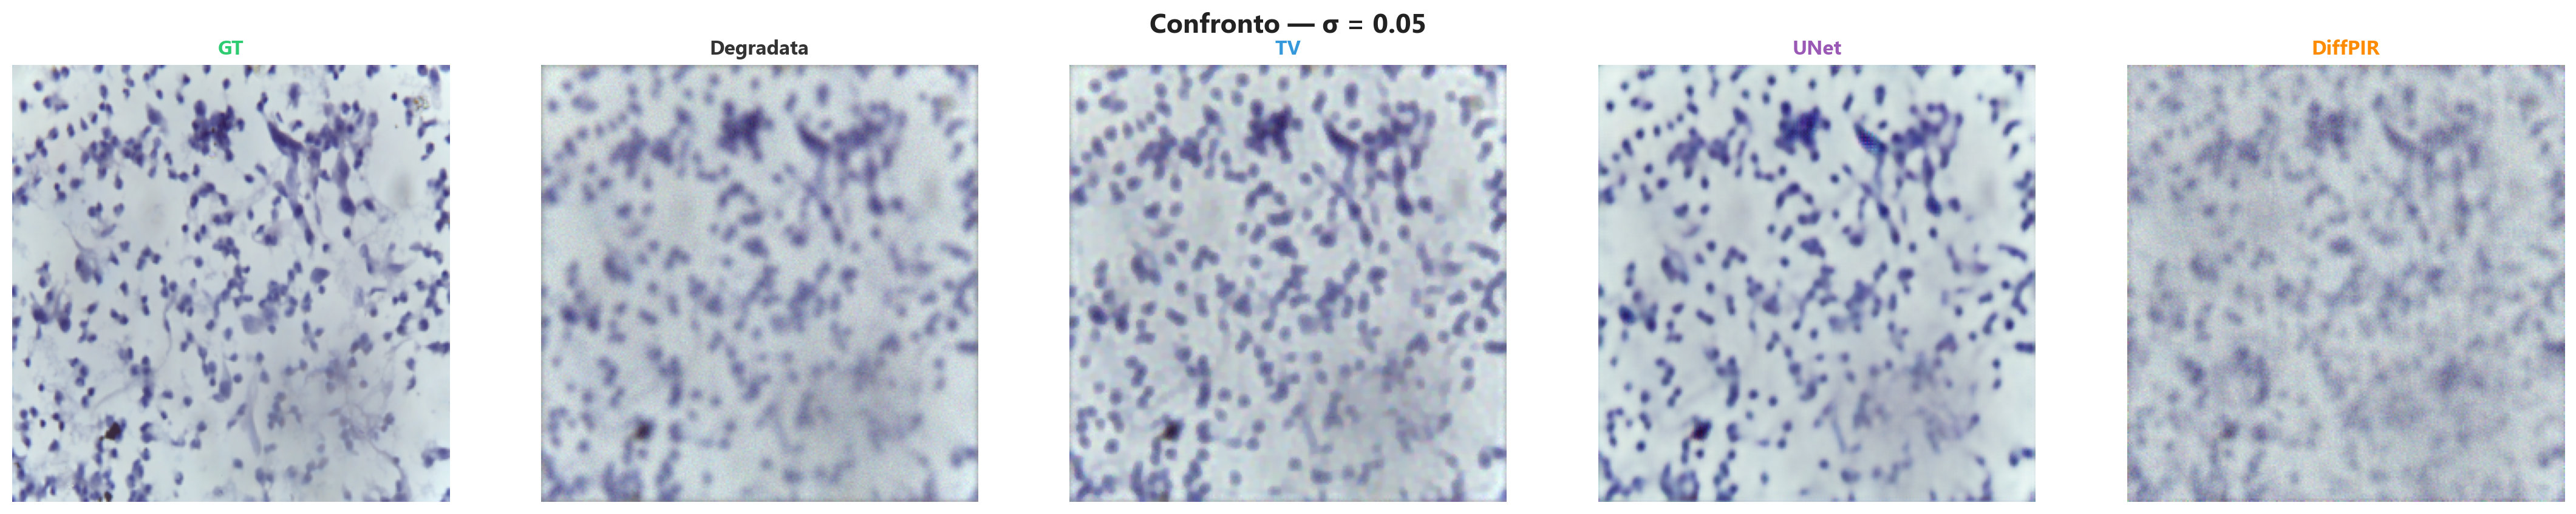
\includegraphics[width=0.74\textwidth]{../results/qualitative_slides/noise_0.05_comparison.png}
  \end{center}
\end{frame}

\begin{frame}[shrink]{Confronto Visivo -- $\sigma_n = 0.1$}
  \begin{center}
    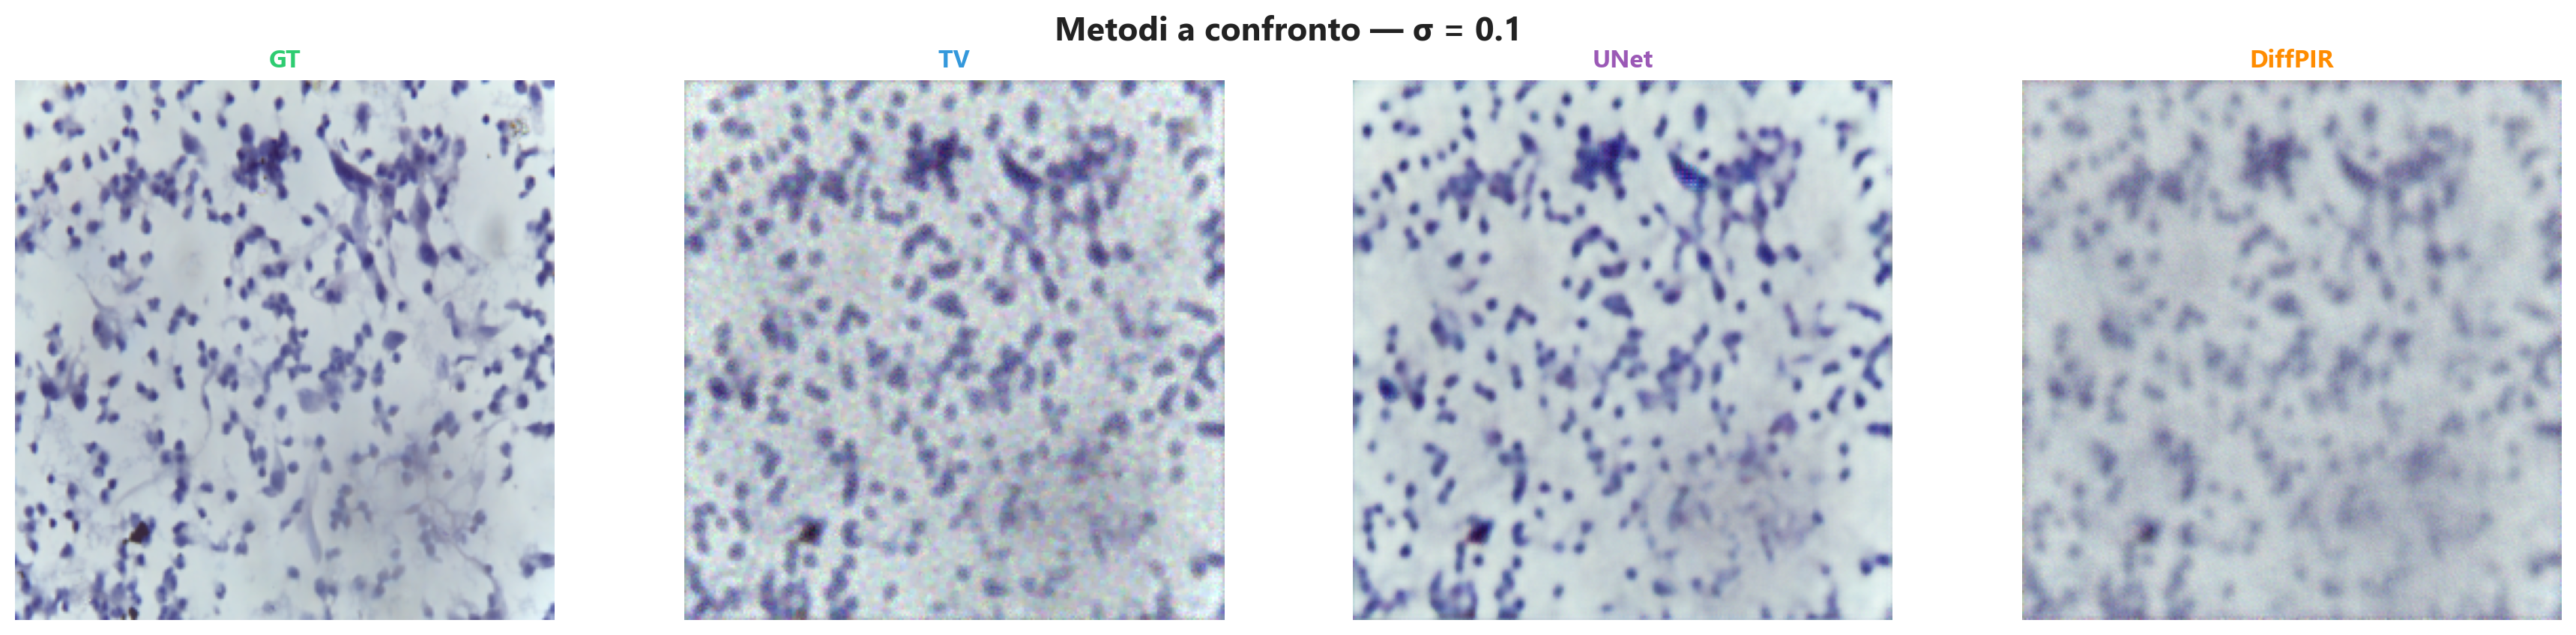
\includegraphics[width=0.80\textwidth]{../results/qualitative_slides/methods_noise_0.1.png}
    \vspace{0.05cm}
    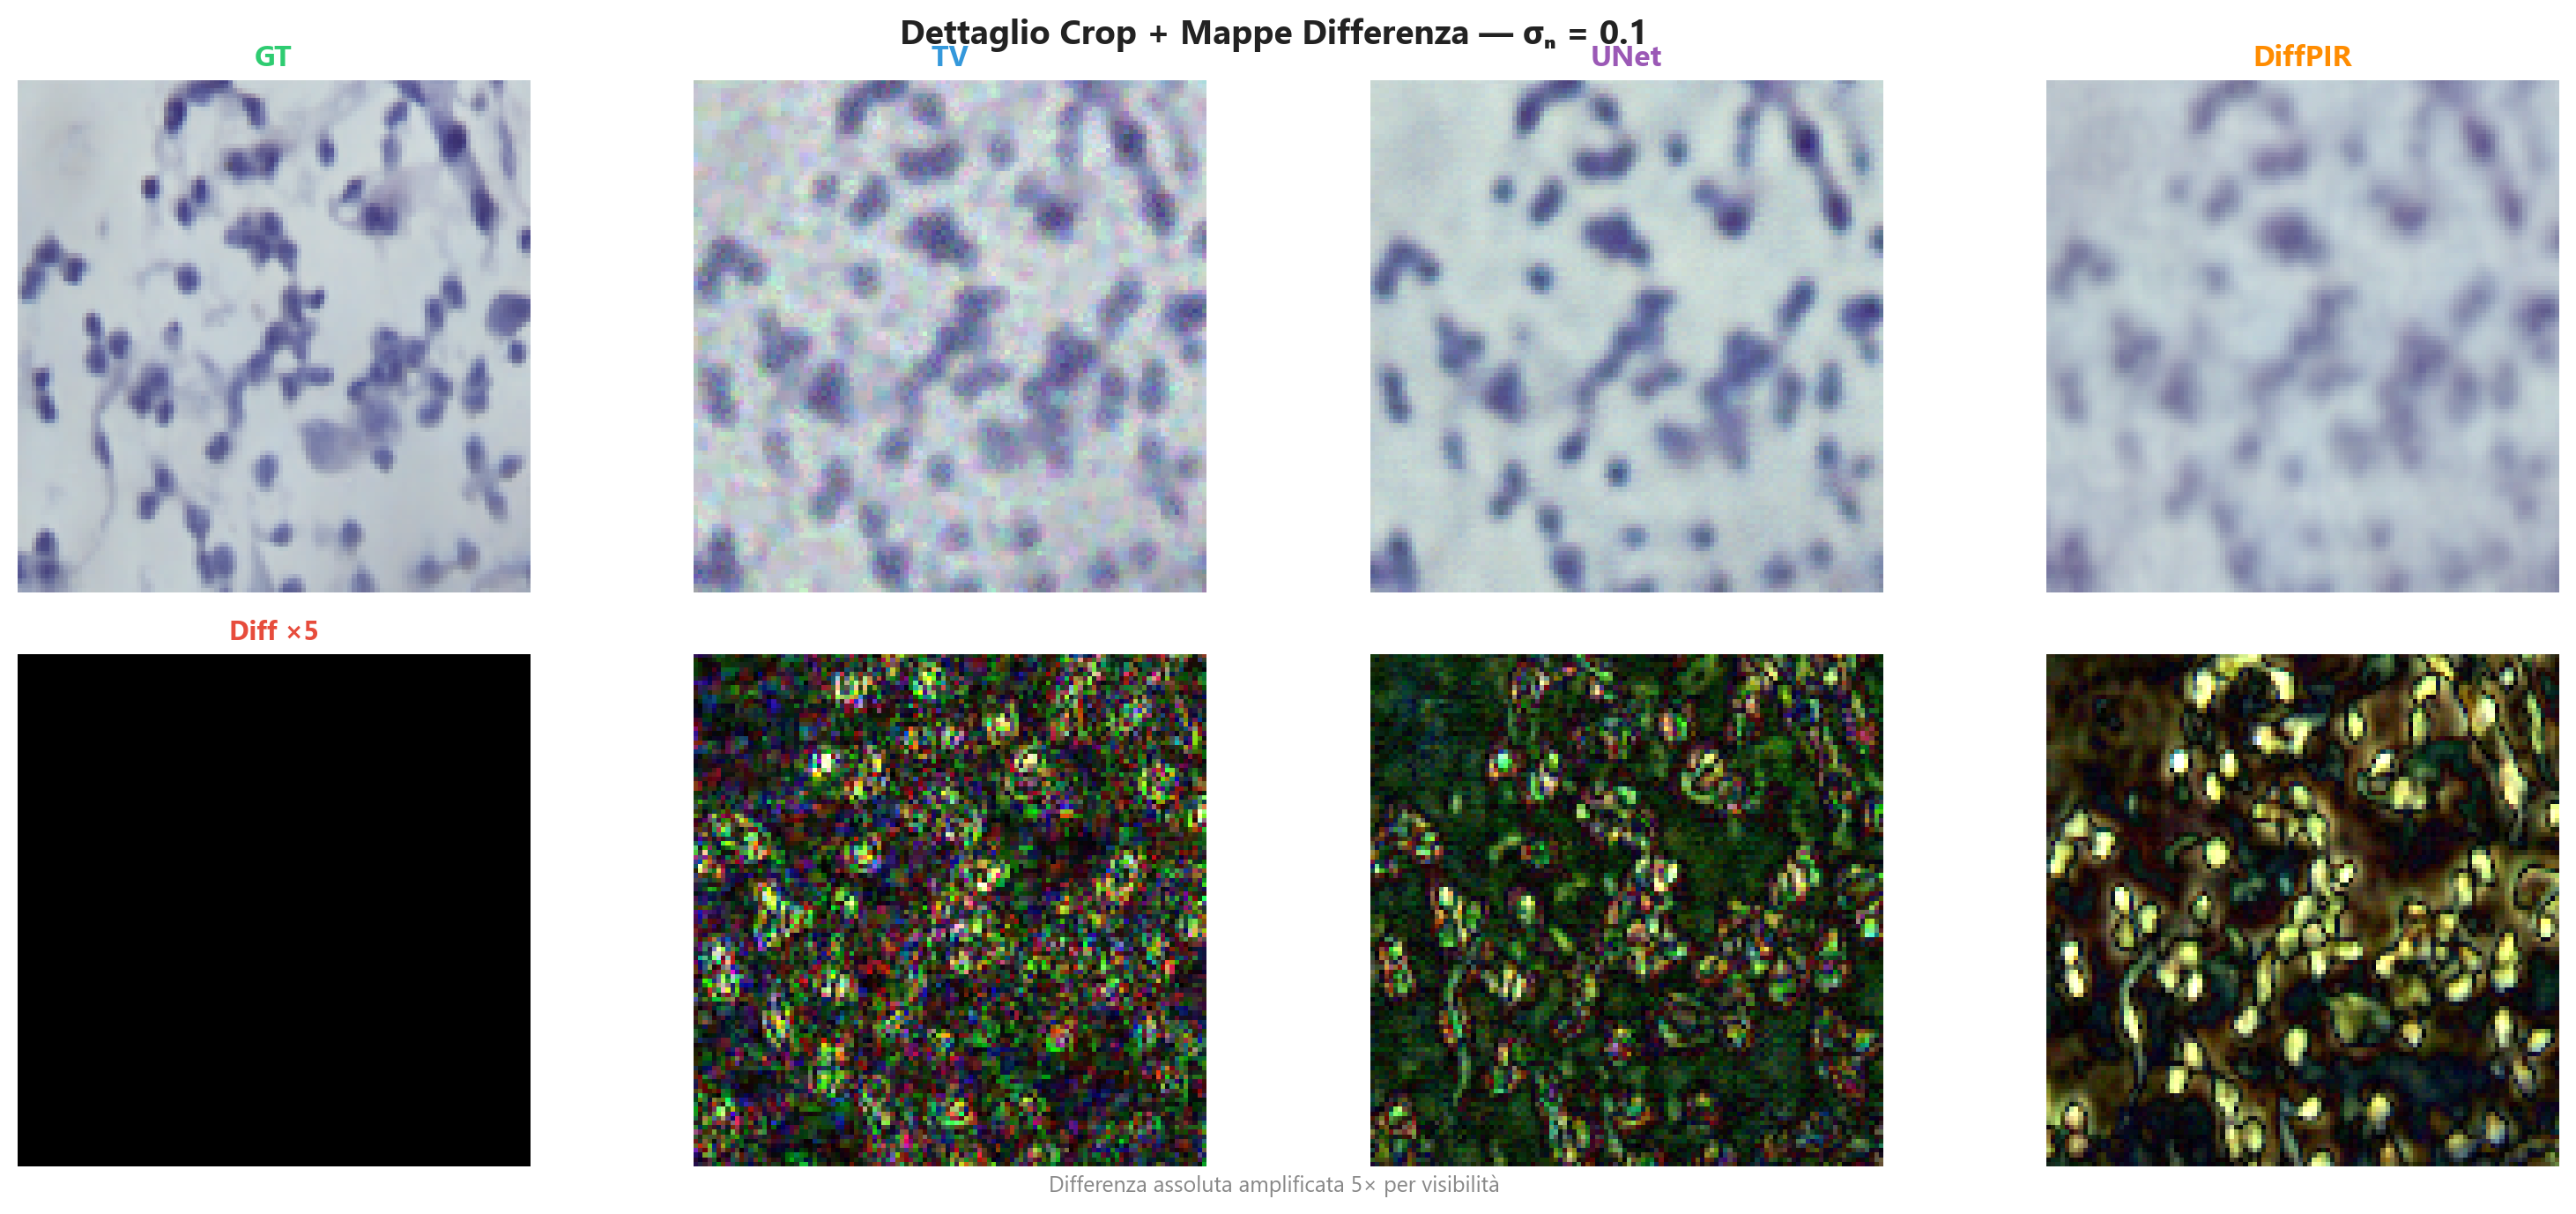
\includegraphics[width=0.55\textwidth]{../results/qualitative_slides/crop_diff_comparison.png}
  \end{center}
  \vspace{0.05cm}
  \begin{center}
    \small\textbf{Mappe di differenza} ($|\hat{x} - x_{\text{GT}}|$, normalizzate)
  \end{center}
  \begin{center}
    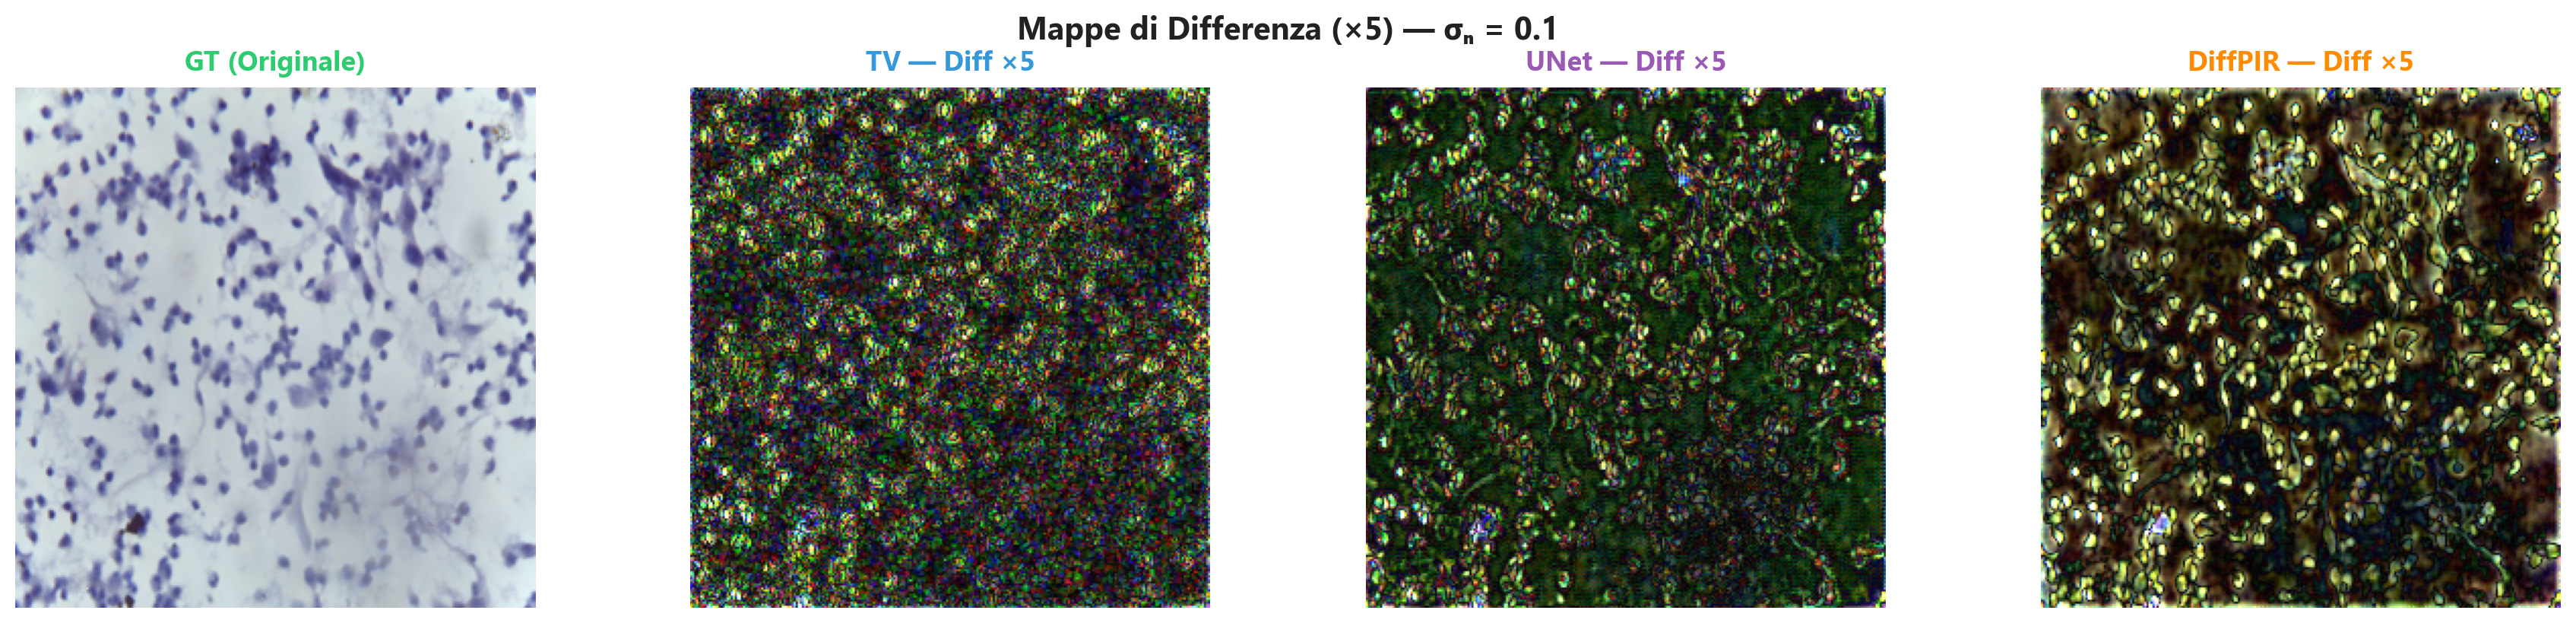
\includegraphics[width=0.65\textwidth]{../results/diff/all_diffs_0.1.png}
  \end{center}
\end{frame}

\section{Discussione}

\begin{frame}{Confronto tra le Famiglie}
  \begin{columns}[t]
    \column{0.48\textwidth}
      {\setbeamercolor{block title}{bg=darkblue,fg=white}%
       \setbeamercolor{block body}{bg=darkblue!5}%
      \begin{block}{\small\bfseries TV  \hfill \scriptsize\itshape Variazionale}
        \scriptsize
        \textcolor{green!50!black}{$\blacktriangleright$} \textbf{Pro}\\[0.05cm]
        \hspace{0.3cm}$\checkmark$ Non richiede dati di training\\
        \hspace{0.3cm}$\checkmark$ Interpretabile, soluzione unica\\
        \hspace{0.3cm}$\checkmark$ Robusto a basso rumore ($\sigma_n \leq 0.01$)\\[0.08cm]
        \textcolor{red}{$\blacktriangleright$} \textbf{Contro}\\[0.05cm]
        \hspace{0.3cm}$\times$ Staircasing a $\lambda$ troppo alto\\
        \hspace{0.3cm}$\times$ Degrada rapidamente ad alto $\sigma_n$
      \end{block}}

    \column{0.48\textwidth}
      {\setbeamercolor{block title}{bg=green!45!black,fg=white}%
       \setbeamercolor{block body}{bg=green!5}%
      \begin{block}{\small\bfseries UNet  \hfill \scriptsize\itshape Deep Learning}
        \scriptsize
        \textcolor{green!50!black}{$\blacktriangleright$} \textbf{Pro}\\[0.05cm]
        \hspace{0.3cm}$\checkmark$ Inferenza velocissima (0.035\,s/img)\\
        \hspace{0.3cm}$\checkmark$ Robusto su tutto lo spettro ($\Delta$PSNR $\sim$1\,dB)\\[0.08cm]
        \textcolor{red}{$\blacktriangleright$} \textbf{Contro}\\[0.05cm]
        \hspace{0.3cm}$\times$ Richiede training supervisionato\\
        \hspace{0.3cm}$\times$ Generalizzazione limitata al dominio
      \end{block}}
  \end{columns}

  \vspace{0.25cm}

  \begin{columns}[t]
    \column{0.70\textwidth}
      {\setbeamercolor{block title}{bg=orange!75!black,fg=white}%
       \setbeamercolor{block body}{bg=orange!5}%
      \begin{block}{\small\bfseries DiffPIR  \hfill \scriptsize\itshape Generativo (Plug-and-Play)}
        \scriptsize
        \textcolor{green!50!black}{$\blacktriangleright$} \textbf{Pro}\\[0.05cm]
        \hspace{0.3cm}$\checkmark$ Ricostruisce dettagli persi dagli altri metodi\\
        \hspace{0.3cm}$\checkmark$ Migliora all'aumentare del rumore (15.78\,$\to$\,25.46\,dB)\\[0.08cm]
        \textcolor{red}{$\blacktriangleright$} \textbf{Contro}\\[0.05cm]
        \hspace{0.3cm}$\times$  Lento ($\sim$3\,s/img) -- 15 step DDIM\\
        \hspace{0.3cm}$\times$  Allucinazioni a basso $\sigma_n$ (inventa dettagli inesistenti)
      \end{block}}
    \column{0.26\textwidth}
      \begin{center}
        \textbf{Metriche chiave}\\[0.15cm]
        \begin{tabular}{rl}\small
          \textbf{TV} & 32.09\,dB\\
          \textbf{UNet} & 29.79\,dB\\
          \textbf{DiffPIR} & 25.46\,dB\\
        \end{tabular}\\[0.1cm]
        \scriptsize (PSNR a $\sigma_n=0.005$)
      \end{center}
  \end{columns}
\end{frame}

\begin{frame}{Regimi di Funzionamento}
  \begin{center}
    \begin{tabular}{lccc}\toprule
      \textbf{Scenario} & \textbf{TV} & \textbf{UNet} & \textbf{DiffPIR}\\\midrule
      Basso rumore ($\sigma_n<0.05$) & \upgreen\ Eccellente & \upgreen\ Buono & \downred\ Scarso\\
      Medio rumore ($\sigma_n=0.05$) & \upgreen\ Buono & \upgreen\ Molto buono & \upgreen\ Adeguato\\
      Alto rumore ($\sigma_n=0.1$)   & \downred\ Mediocre & \upgreen\ \textbf{Migliore} & \upgreen\ Buono\\
      Velocit\`a inferenza           & $\sim$7 s & $\sim$\textbf{0.035 s} & $\sim$3 s\\\bottomrule
    \end{tabular}
  \end{center}
  \vspace{0.3cm}
  \begin{block}{Nessun metodo domina tutti i regimi}
    \begin{itemize}
      \item Scelta dipende dal contesto applicativo
      \item UNet: miglior compromesso complessivo
      \item DiffPIR: utile solo ad alto rumore
      \item TV: scelta pragmatica a basso rumore
    \end{itemize}
  \end{block}
\end{frame}

\section{Conclusioni}

\begin{frame}{Conclusioni}
  \begin{block}{Risultati Principali}
    \begin{itemize}
      \item Confronto \textbf{equo} di 3 famiglie metodologiche
      \item Pipeline unica, stesse metriche, stesso test set
      \item \textbf{34 test unitari} di verifica
    \end{itemize}
  \end{block}
  \begin{block}{Lezioni Apprese}
    \begin{itemize}
      \item Ill-posed non significa irrisolvibile: compromessi diversi
      \item Generativi con cautela a basso rumore
      \item CPU limita scala sperimentale
    \end{itemize}
  \end{block}
  \begin{block}{Direzioni Future}
    \begin{itemize}
      \item Tuning adattivo $\lambda(\sigma_n)$ per TV
      \item Training GPU per modelli pi\`u grandi
      \item Validazione su immagini cliniche reali
    \end{itemize}
  \end{block}
\end{frame}

\section{Bibliografia}

\begin{frame}{Riferimenti}
  \footnotesize
  \begin{thebibliography}{10}
    \bibitem{diffpir} Y. Zhu et al., \emph{Denoising Diffusion Models for Plug-and-Play Image Restoration}, CVPR 2023.
    \bibitem{ddpm} J. Ho et al., \emph{Denoising Diffusion Probabilistic Models}, NeurIPS 2020.
    \bibitem{ddim} J. Song et al., \emph{Denoising Diffusion Implicit Models}, ICLR 2021.
    \bibitem{tv} L. Rudin, S. Osher, E. Fatemi, \emph{Nonlinear total variation based noise removal algorithms}, Physica D 1992.
    \bibitem{unet} O. Ronneberger et al., \emph{U-Net: Convolutional Networks for Biomedical Image Segmentation}, MICCAI 2015.
    \bibitem{data} Mendeley LBC Cervical Cancer, \href{https://data.mendeley.com/datasets/zddtpgzv63/2}{doi: 10.17632/zddtpgzv63.2}
  \end{thebibliography}
  \vspace{0.5cm}
  \begin{center}
    \Large\textcolor{darkblue}{\textbf{Grazie per l'attenzione!}}
  \end{center}
\end{frame}

\end{document}